\documentclass[12pt]{report}
\usepackage[utf8]{inputenc}
\usepackage{geometry}
\geometry{letterpaper, margin=0.25in}
\usepackage{graphicx} 
\usepackage{multicol}
\usepackage{parskip}
\usepackage{booktabs}
\usepackage{array} 
\usepackage{paralist} 
\usepackage{verbatim}
\usepackage{sectsty}
\usepackage[shortlabels]{enumitem}

\usepackage{amsmath}
\usepackage{amssymb}
\usepackage{mathtools}
\usepackage{empheq}
\usepackage{xcolor}
\usepackage{bbm}
\usepackage{tikz}
\usepackage{pgfplots}
\usepackage{tikz-cd}
\usepackage{circuitikz}
\usepackage{multirow}

\pgfplotsset{compat=1.18}
\usetikzlibrary{intersections, decorations.markings, decorations.pathmorphing, patterns}
 \usepgfplotslibrary{fillbetween}
\tikzset{
    marking along/.style n args={2}{
        decoration={
                markings, 
                mark=at position #1 with {\arrow{#2}}
        },
        postaction={decorate}
        },
    marking along/.default={0.5}{>},
    wavy/.style={
        decorate,decoration={coil,aspect=0}
     },
    two marks/.style n args={1}{
        decoration={
            markings,
            mark=at position 0.25 with {\arrow{#1}},
            mark=at position 0.75 with {\arrow{#1}}
         },
         postaction={decorate}
    },
    two marks/.default={>}
}

\colorlet{mygreen}{green!50!teal}
\colorlet{darkblue}{blue!60!black}

\newcommand{\ans}[1]{\boxed{\text{#1}}}
\newcommand{\vecs}[1]{\langle #1\rangle}
\renewcommand{\hat}[1]{\widehat{#1}}

\renewcommand{\P}{\mathbb{P}}
\newcommand{\R}{\mathbb{R}}
\newcommand{\E}{\mathbb{E}}
\newcommand{\Z}{\mathbb{Z}}
\newcommand{\N}{\mathbb{N}}
\newcommand{\Q}{\mathbb{Q}}
\newcommand{\C}{\mathbb{C}}

\newcommand{\ind}{\mathbbm{1}}
\newcommand{\qed}{\quad \blacksquare}

\newcommand{\brak}[1]{\left\langle #1 \right\rangle}
\newcommand{\bra}[1]{\left\langle #1 \right\vert}
\newcommand{\ket}[1]{\left\vert #1 \right\rangle}

\newcommand{\abs}[1]{\left\vert #1 \right\vert}
\newcommand{\norm}[1]{\left\vert \left\vert #1 \right\vert \right\vert}

\newcommand{\mfX}{\mathfrak{X}}
\newcommand{\ep}{\varepsilon}

\newcommand{\Ec}{\mathcal{E}}
\newcommand{\Nc}{\mathcal{N}}
\newcommand{\A}{\mathcal{A}}
\newcommand{\F}{\mathcal{F}}
\newcommand{\Cc}{\mathcal{C}}
\newcommand{\B}{\mathcal{B}}
\newcommand{\M}{\mathcal{M}}
\newcommand{\X}{\chi}
\renewcommand{\L}{\mathcal{L}}

\newcommand{\sub}{\subseteq}
\newcommand{\st}{\text{ s.t. }}
\newcommand{\card}{\text{card }}
\renewcommand{\div}{\vspace*{10pt}\hrule\vspace*{10pt}}
\newcommand{\surj}{\twoheadrightarrow}
\newcommand{\inj}{\hookrightarrow}
\newcommand{\biject}{\hookrightarrow \hspace{-8pt} \rightarrow}
\renewcommand{\bar}[1]{\overline{#1}}
\newcommand{\overcirc}[1]{\overset{\circ}{#1}}
\newcommand{\diam}{\text{diam }}
\newcommand{\iid}{\overset{\text{iid}}{\sim}}

\renewcommand{\Re}{\text{Re}\,}
\renewcommand{\Im}{\text{Im}\,}
\newcommand{\Var}{\text{Var}\,}
\newcommand{\Cov}{\text{Cov}\,}

\DeclareMathOperator*{\argmax}{\arg\max}
\DeclareMathOperator*{\argmin}{\arg\min}
\DeclareMathOperator*{\Unif}{\text{Unif}\,}


\newcommand{\sign}{\text{sign}\,}

\newcommand*{\tbf}[1]{\ifmmode\mathbf{#1}\else\textbf{#1}\fi}


\usepackage{tcolorbox}
\tcbuselibrary{breakable, skins}
\tcbset{enhanced}
\newenvironment*{tbox}[2][gray]{
    \begin{tcolorbox}[
        parbox=false,
        colback=#1!5!white,
        colframe=#1!75!black,
        breakable,
        title={#2}
    ]}
    {\end{tcolorbox}}

\newenvironment*{exercise}[1][red]{
    \begin{tcolorbox}[
        parbox=false,
        colback=#1!5!white,
        colframe=#1!75!black,
        breakable
    ]}
    {\end{tcolorbox}}

\newenvironment*{proof}[1][blue]{
\begin{tcolorbox}[
    parbox=false,
    colback=#1!5!white,
    colframe=#1!75!black,
    breakable
]}
{\end{tcolorbox}}
\newenvironment*{proposition}[1][gray]{
    \begin{tcolorbox}[
        parbox=false,
        colback=#1!5!white,
        colframe=#1!75!black,
        breakable
    ]}
    {\end{tcolorbox}}


\title{ ENGN 1580 - Communications Systems}
\author{Milan Capoor}
\date{Spring 2026}

\begin{document}
\maketitle

\chapter{Fourier Transforms}
\section{Jan 22}

\subsection{Linear Systems}

What is a linear system? 
\begin{enumerate}
    \item $L[u+v] = L[u]+L[v]$ (additivity)
    \item $L[au] = aL[u]$ (scaling) 
    \item $L[ax + by] = aL[x] + bL[y]$ (superposition)
\end{enumerate}

Do we actually need scaling if we have additivity?

\emph{Example 1.} 
\[ L[x+x]= Lx + Lx = 2Lx \]
seems like  we don't. What about rationals?

\emph{Example 2.} if we want $L[0.1x]$ we can see 
\[L[x]= L[0.1x + \dots + 0.1x] = 10L[0.1x] \implies L[0.1x] = \frac{1}{10}L[x] \]
still working... 

\emph{Example 3.} And even for negatives...
\begin{gather*}
    L[-x]=L[x-x-x]=L[x]+2L[-x]
    0 = L[x]+L[-x]
    L[-x] = -L[x]
\end{gather*}

(\tbf{Remark:} this also immediately leads to the identity $L[0]=0$ for all linear systems)

\emph{Example 4 (A counter):} What if $L[ax]$ is irrational? We can approximate by rationals and apply the same arguments above but this requires $L$ continuous on $\R \setminus \Q$ -- a rather strong condition 

Where things really break are $\C$: what could we possibly say about $L[jx]$? (convention: $j$ is imaginary basis in this class)

\subsection{Periodic Signals}

\tbf{Signal:} a function 

\tbf{periodic signals:} from fourier series 
\[p(t) = \sum p_k exp(2\pi jk/T) \]
for period $T$ 
where 
\[p_k = \frac 1T \int_{-T/2}^{T/2} p(t) e^{-j * 2\pi /T * kt} \; dt\]
(as an aside notice that this is a projection) 

\tbf{Fourier transform:}
\[\mathfrak X f = \int x(t) e^{-j * 2\pi ft} \; dt \]

\tbf{Inverse Fourier:}
\[x(t) = \int \mathfrak Xf e^{j* 2\pi ft} \; df\]

where $f$ is the frequency (note we are missing the coefficients because we work in Hz) 

\tbf{Laplace:}
\[x(s) = \int x(t) e^{-st} \; dt \]

Notice that all of these transforms have integrals of exponentials. Why might that be? 

\tbf{Linear time invariant (LTI) systems:} Let L[x(t)] = y(t). If this is an LTI,
\[L[x(t-\tau)] = y(t - \tau)\]

\tbf{impulse:} square function of lengths $1/\ep$ centered at 0 satisfying 
\begin{enumerate}
    \item $\int \delta(t) \; dt = 1 $
    \item $\int \delta(t-a)s(t) \; dt = s(a) $(sifting property) 
\end{enumerate}

\begin{center}
\begin{tikzpicture}
    \draw (0, 0) -- (4, 0);
    \draw (2, 0) -- (2, 3);
    \draw[blue] (1, 0) rectangle ++(2, 2);

    \node[below] at (1, 0) {$-\ep/2$};
    \node[below] at (3, 0) {$\ep/2$};
    \node[right] at (3, 2) {$1/\ep$};
    
\end{tikzpicture}
\end{center}

This leads to an alternative definition of an LTI $h(t)$ as one for which 
\begin{enumerate}
    \item $h(\delta(t)) = h(t)$
    \item $h(a\delta(t-\tau)) =ah(t-\tau)$
\end{enumerate}

Let us consider a general case 
\[x(t) = \int x(\tau)\delta(t-\tau)d\tau\]
now what is $h(x(t))$? 

If we view the integral as a Riemann sum, we can see easily that 
\begin{align*}
    h(x(t)) &= h(\int x(\tau)\delta(t-\tau)d\tau)\\ 
    &= \int x(\tau)h(t-\tau)d\tau \\ 
    &= y(t)
\end{align*}
a convolution! (and of course we could equally see by a change of variables $\int x(t-\tau)h(\tau)d\tau$)

What about $h(e^{jst})$? 
\[\int e^{js(t-\tau)} h(\tau) d\tau= e^{jst} \int h(t) e^{-jst} d\tau\]

\section{Jan 27}

\tbf{Outline of a Communications System:}
\begin{center}
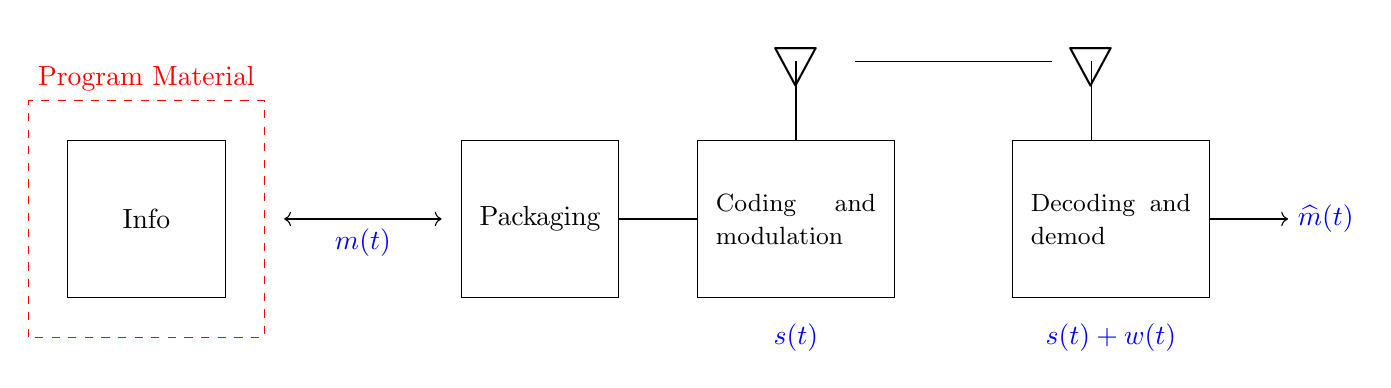
\begin{tikzpicture}

    \draw (-1, 0) rectangle ++(2, 2) node[midway] {Info};
    \draw[red, dashed] (-1.5, -0.5) rectangle ++(3, 3) node[above left] {Program Material};

    \draw[<->] (1.75, 1) -- ++(2, 0) node[midway, below, blue] {$m(t)$};
    \draw (4,0) rectangle ++(2, 2) node[midway] {Packaging};
    \draw (6, 1) -- (7, 1);
    \draw (7,0) rectangle ++(2.5, 2) node[midway] {\parbox{0.8in}{{\small Coding and modulation}}};
    \draw (8.25, 2) -- ++(0, 1) node {\rotatebox{180}{\scalebox{2}{$\triangle$}}};
    \node[blue] at (8.25, -0.5) {$s(t)$};

    \draw (9, 3) to[decorate, decoration={coil, aspect=2}] ++(2.5, 0) ;

    \draw (12, 2) -- ++(0, 1) node {\rotatebox{180}{\scalebox{2}{$\triangle$}}};
    \draw (11,0) rectangle ++(2.5, 2) node[midway] {\parbox{0.8in}{{\small Decoding and demod}}};
    \node[blue] at (12.25, -0.5) {$s(t) + w(t)$};

    \draw[->] (13.5, 1) -- ++(1, 0) node[blue, right] {$\hat m(t)$};

\end{tikzpicture}
\end{center}
where: 
\begin{itemize}
    \item info is viewed broadly as songs, video, text, etc.
    \item $m(t)$ is the message signal (assuming no loss between program material and packaging)
    \item $s(t)$ is the transmitted signal
    \item $w(t)$ is noise added by the transmission interference 
    \item $\hat m(t)$ is the received (estimated) message signal
\end{itemize}

\subsection{Linear system review:}
A system $L$ is \tbf{linear} if it satisfies \emph{superposition}: 
\[L{ax + by} = aL[x] + bL[y]\]

If we define a delta function $\delta(t)$ satisfying
\begin{enumerate}
    \item $\int_{-\infty}^{\infty} \delta(t)\; dt = \int_{0^-}^{0^+} \delta(t) \; dt = 1$
    \item $\int \delta(t-a)s(t) \; dt = s(a)$ (sifting property)
\end{enumerate}

Last time we saw the square pulse. However, we can also define it as the limit of a Gaussian as $\sigma \to 0$: 
\[\delta_{\sigma}(t) = \sqrt{\frac{1}{2\pi\sigma^2}} e^{-\frac{t^2}{2\sigma^2}}\]

\begin{center}
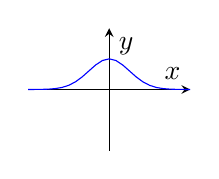
\begin{tikzpicture}
\begin{axis}[
    width=0.3\textwidth,
    axis lines=middle,
    no markers,
    xtick=\empty,
    ytick=\empty,
    clip=false,
    xlabel={$x$},
    ylabel={$y$},
    domain=-2:2,
    ymin=-2, ymax=2,
    xmin= -2, xmax=2,
    view = {0}{90}
]
    \addplot{exp(-x^2/0.5)};
\end{axis}
\end{tikzpicture}
\end{center}

\begin{exercise}
    \textbf{Exercise:} Show that $\delta_{\sigma}(t)$ is a delta function as $\sigma \to 0$. 
\end{exercise}

\tbf{Impulse response of a linear system:} 

\begin{center}
\begin{tikzpicture}
    \draw (0, 0) rectangle ++(2, 2) node[midway] {$h(t)$}; 
    \draw[<-, shorten <= 5pt] (0, 1) -- ++(-1,  0) node[left] {$\delta(t -t_0)$}; 
    \draw[->, shorten <= 5pt] (2, 1) -- ++(1, 0) node[right] {$h(t- t_0)$};
\end{tikzpicture}
\end{center}

With a little work, we can generalize this property to see that for any input signal $x(t)$, the output of a linear system is given by the convolution of the input with the impulse response:

\begin{align*}
    y(t) &= h(x(t)) \\
    &= \int_{-\infty}^{\infty} x(\tau) h(t - \tau) \; d\tau \\
    &= \int_{-\infty}^{\infty} x(t- \tau) h(\tau) \; d\tau
\end{align*}

\tbf{Fourier Transform:}
\[h(t) \overset{\F}{\implies} H(f) = \int_{-\infty}^{\infty} h(t) e^{-j\;2\pi ft}\; dt\]

\emph{Example:} Let $x(t) = \cos 2\pi f_0 t$. What is $X(f)$?
\begin{align*}
    \cos 2\pi f_0 t &= \frac{e^{j\; 2\pi f_0t} + e^{-j\; 2\pi f_0t}}{2}\\ 
    h(\cos 2\pi f_0t) &= \frac{1}{2}h(e^{j\; 2\pi f_0t}) + \frac{1}{2}h(e^{-j\; 2\pi f_0t}) \\
    &= \frac{1}{2}e^{j\; 2\pi f_0t}H(f_0) + \frac{1}{2}e^{-j\; 2\pi f_0t}H(-f_0)
\end{align*}

Let's generalize: 
\begin{align*}
    h(x(t)) &= y(t) - \int x(\tau) h(t - \tau) \; d\tau \\
    &\overset{\F}{=} \int \int x(\tau) h(t - \tau) e^{-j\; 2\pi ft} \; dt\, d\tau\\
    &= \int x(\tau) \left(\int h(t -\tau) e^{-j\; 2\pi ft}\; dt\right) \; d\tau\\ 
    &= \int x(t) \left[\int h(u) e^{-j\; 2\pi f(u + \tau)}\right]\; d\tau \qquad (u = t -\tau)\\ 
    &=  \int x(t) \underbrace{\left[\int h(u) e^{-j\; 2\pi fu}\right]}_{H(f)} e^{-j\; 2\pi f\tau}\; d\tau\\
    &\overset{\F^{-1}}= X(f)H(f)
\end{align*}

Which yields the important result: \emph{convolution in the time domain is multiplication in the frequency domain:}
\[x(t) \star h(t) = (x\star h)(t) \overset{\F}{=} X(f)H(f)\]

In fact, the work here leads to a number of useful properties of the Fourier transform:

\tbf{Time shift property:} 
\[\boxed{\F[x(t- t_0)] = e^{j\; 2\pi ft_0} X(f)}\]

\tbf{Scaling:} 
\begin{align*}
    \F[x(at)] &= \int x(at) e^{-j\; 2\pi ft}\; dt\\ 
    &= \int x(u) e^{-j\; 2\pi f(u/a)} \frac{du}{a} \qquad (du = a\; dt)\\
    &= \boxed{\frac{1}{\abs a} X(f/a) }
\end{align*}

\tbf{Differentiation:}
\begin{align*}
    \frac{d}{dt} x(t) &= \frac{d}{dt}\left[\int X(f) e^{j\; 2\pi ft}\; df\right] \\ 
    &= \int X(f)(j\; 2\pi f) e^{j\; 2\pi ft}\; dt
\end{align*}
so 
\[\boxed{\F\left[\frac{dx}{dt}\right] = X(f) \; j 2\pi f}\]

\tbf{Integration:}
\[\boxed{\F\left[\int_{-\infty}^t x(u)\; du\right] = \frac{X(f)}{j\, 2\pi f} + \frac{X(0)}{2} \delta(f)}\]

\begin{exercise}
    \textbf{Exercise:} Prove the integration property
\end{exercise}

\tbf{Parseval:}
\[\boxed{\int_{-\infty}^{\infty} x^2(t) = \Ec_x = \int_{-\infty}^{\infty} \abs{X(f)}^2 \; df}\]
(``the energy in time domain = energy in frequency domain'')

We've seen over and over that $\F[x(t)] = X(f)$? What about $\F[X(f)]$? 

First, two fact that should be obvious:
\begin{align*}
    \F[\delta(t)] &= 1\\ 
    \F[\delta(t - \tau)] &= e^{-j\; 2\pi ft}
\end{align*}
and since (up to sets of measure zero), 
\[\delta(t - \tau) \overset{\F}{\underset{\F^{-1}}{\iff}} e^{-j\; 2\pi ft}\]

which gives us 

\tbf{Duality:}
\begin{align*}
    \F[X(t)] &= \int X(t) e^{-j\; 2\pi ft}\; dt\\ 
    &= \int x(u) e^{-j\; 2\pi(-tu)} \; du\\ 
    &= \int \int x(u) e^{-j\; 2\pi tu} e^{-j\; 2\pi t}\; du\, dt\\
    &= \int x(u) \left[\int e^{-j\; 2\pi t(u+f)}\; dt\right] \; du\\ 
    &= \int x(u) \delta(u + f)\; du\\
    &= x(-f)
\end{align*}

Graphically, for a square function, 

\begin{center}
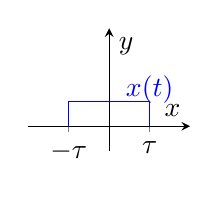
\begin{tikzpicture}
\begin{axis}[
    width=0.3\textwidth,
    axis lines=middle,
    no markers,
    xtick={-2, 2},
    xticklabels={$-\tau$, $\tau$},
    ytick={\empty},
    clip=false,
    xlabel={$x$},
    ylabel={$y$},
    domain=-2:2,
    ymin=-1, ymax=4,
    xmin= -4, xmax=4,
    view = {0}{90}
]

\addplot coordinates {(-2, 0) (-2, 1) (2, 1) (2, 0)};
\node[blue] at (2, 1.5) {$x(t)$};
\end{axis}
\end{tikzpicture}
\end{center}

\begin{align*}
    \F[x(t)] &= \int_{-T}^T e^{-j\; 2\pi ft} \;dt\\ 
    &= \left(\frac{1}{-j\, 2\pi f}\right) e^{-j\; 2\pi ft} \bigg\vert_{-T}^T\\ 
    &= -\frac{1}{j\, 2\pi f} \left(e^{-j\; 2\pi fT} - e^{j\; 2\pi fT}\right)  \\ 
    &= -\frac{1}{\pi f} \sin(-2\pi fT)  \qquad \left(\sin z = \frac{e^{jz} - e^{-jz}}{2j}\right) \\ 
    &= \frac{\sin 2\pi fT}{\pi f} \\ 
\end{align*}

\begin{center}
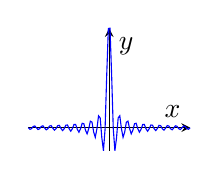
\begin{tikzpicture}
\begin{axis}[
    width=0.3\textwidth,
    axis lines=middle,
    no markers,
    xtick=\empty,
    ytick=\empty,
    clip=false,
    xlabel={$x$},
    ylabel={$y$},
    domain=-2*pi:2*pi,
    samples=100,
    view = {0}{90}
]
    \addplot {sin(10*deg(x))/(7*x)};
\end{axis}
\end{tikzpicture}
\end{center}

\section{Jan 29}

\tbf{Recall:} What is the Fourier transform of this box? 

\begin{center}
\begin{tikzpicture}
    \draw (0, 0) -- (6, 0);
    \draw (3, 0) -- (3, 3);

    \draw[blue] (1, 0) node[below] {$-T/2$} -- (1, 2) -- (5, 2) node[above right] {$1/T$} -- (5, 0) node[below] {$T/2$};
\end{tikzpicture}
\end{center}

(Note this is an impulse as $T \to 0$)

\[\F = \int_{-T/2}^{T/2} \frac{1}{T} e^{-j\; 2\pi ft}\; dt = \frac{1}{T} \left(\frac{1}{-j\, 2\pi f}\right) e^{-j\; 2\pi ft} \bigg\vert_{-T/2}^{T/2} = \frac{1}{-j\, 2\pi f T} \left(e^{-j\; \pi f T} - e^{j\; \pi f T}\right) = \frac{\sin(\pi f T)}{\pi f T} \]

How might we sanity check this? 

We already saw that as $T \to 0$, this becomes an impulse in the time domain. What happens in the frequency domain?
\[\lim_{T \to 0} \frac{\sin \pi f T}{\pi f T} = 1\]
and indeed this matches the rule $\F(\delta(t)) = 1$.

\emph{Example:} 
\[\F[e^{-at}u(t)] = \int_0^{\infty} e^{-at} e^{-j\; 2\pi ft}\; dt
    = \int_0^{\infty} e^{-(a + j\; 2\pi f)t}\; dt
    = \frac{1}{a + j\; 2\pi f}
\]
(for $a > 0$ and $u(t)$ the unit step function)

\tbf{Convolution:} 
\[\int_{-\infty}^{\infty} x(\tau) y(t -\tau)\; d\tau\]

\emph{Example:} Convolve two box functions of width $2$:

\begin{center}
\begin{tikzpicture}[scale=0.7]
    \draw (0, 0) -- (6, 0);
    \draw (3, 0) -- (3, 3);

    \draw[blue] (1, 0) node[below] {$-1$} -- (1, 2) -- (5, 2) node[above right] {$x(t)$} -- (5, 0) node[below] {$1$};

    \node at (7, 1) {\scalebox{2.5}{$\star$}};

    \draw (8, 0) -- (14, 0);
    \draw (11, 0) -- (11, 3);

    \draw[red] (9, 0) node[below] {$-1$} -- (9, 2) -- (13, 2) node[above right] {$y(t)$} -- (13, 0) node[below] {$1$};
\end{tikzpicture}
\end{center}

We could do this directly or we can think about it geometrically.

$y(t - \tau)$ corresponds to a reflection and shift by $t$. 

\begin{center}
\begin{tikzpicture}[scale=0.7]
    \draw (-6, 0) -- (6, 0);
    \draw (3, 0) -- (3, 3);

    \draw[blue] (1, 0) node[below] {$-1$} -- (1, 2) -- (5, 2) node[above right] {$x(t)$} -- (5, 0) node[below] {$1$};

    \draw[red] (-5, 0) node[below] {$t-1$} -- (-5, 2) -- (-1, 2) node[above] {$y(t)$} -- (-1, 0) node[below] {$t+1$};
\end{tikzpicture}
\end{center}

Clearly, multiplying these two functions will give nonzero output only when they overlap. When do they overlap? Precisely at $t \in (-2, 2)$.

\begin{center}
\begin{tikzpicture}
     \draw (-3, 0) -- (3, 0);
    \draw (0, 0) -- (0, 3);

    \draw (-2, 0) node[below] {$-2$} -- (0, 2) node[above right] {$2$} -- (2, 0) node[below] {$-2$};
\end{tikzpicture}
\end{center}

Notice that the length of the domain was 2 before convolving and 4 after convolving. This makes sense since convolution is a ``spreading and smoothing'' operation 

\emph{Example:} $\delta(t) \star x(t)$ where $x(t)$ 

\begin{center}
\begin{tikzpicture}
    \draw (-3, 0) -- (3, 0);
    \draw (0, -2) -- (0, 2);

    \draw[blue] plot[smooth, tension=2] coordinates {(-2, 0) (-1.5, -0.25) (-1, 1) (0, 0) (1, -1) (2, 0)} node[above right] {$x(t)$};
\end{tikzpicture}
\end{center}

Trick question! 
\[\int \delta(x - \tau) x(\tau) \; d\tau = x(t)\]
(sifting!) 

For this class, we should think about convolutions critically and graphically: 

\begin{center}
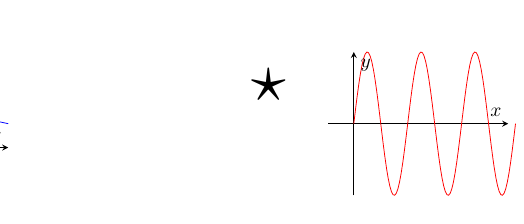
\begin{tikzpicture}[scale=0.7]
    \hspace{-1in}\begin{axis}[
        width=0.4\textwidth,
        axis lines=middle,
        no markers,
        xtick=\empty,
        ytick=\empty,
        clip=false,
        xlabel={$x$},
        ylabel={$y$},
        domain=-2:2,
        ymin=-1, ymax=2,
        xmin= -1, xmax=2,
        view = {0}{90}
    ]

    \addplot[domain=0.4:2, blue] {1/x};
    \end{axis}

    \node at (8, 2) {\scalebox{2.5}{$\star$}};

    \hspace{2.5in}\begin{axis}[
        width=0.4\textwidth,
        axis lines=middle,
        no markers,
        xtick=\empty,
        ytick=\empty,
        clip=false,
        xlabel={$x$},
        ylabel={$y$},
        xmin=-1, xmax=6,
        ymin=-1, ymax=1,
        view = {0}{90}
    ]

    \addplot[domain=0:2*pi, samples=100, red] {sin(3*deg(x))};
    \end{axis}
\end{tikzpicture}
\end{center}

What is the convolution of these two functions at $t= -2$? 

These would be quite annoying to do directly but if we notice that $\textcolor{blue}{x(t)}$ is undefined for $t \leq 0$ then we can see that there is no overlap at all and the convolution is 0.

\begin{proposition}
    \textbf{Recall:} 
    \begin{align*}
        \F(x(t)) &= X(f)\\ 
        \F(X(t)) &= x(-f)\\ 
        \F(\delta(t)) &= 1
    \end{align*}
    so 
    \begin{align*}
        \F(\delta(t- t_0)) &= e^{-j\; 2\pi ft_0}\\ 
        \F(e^{-j\; 2\pi f_0t}) &= \delta(f+ f_0)
    \end{align*}
\end{proposition}

\emph{Example:} $\F(\cos 2\pi f_0 t)$ does not converge analytically BUT 

\[\cos 2\pi f_0 t = \frac{e^{j\; 2\pi f_0t} + e^{-j\; 2\pi f_0t}}{2}\]
so from the above, 

\begin{center}
\begin{tikzpicture}
    \draw (-3, 0) -- (3, 0);
    \draw (0, -1) -- (0, 2);
    \draw (-0.1, 1) -- (0.1, 1) node[above right] {$1/2$};

    \draw[blue, <-] (-2, 1) -- (-2, 0) node[below] {$-f_0$};
    \draw[blue, <-] (2, 1) -- (2, 0) node[below] {$f_0$};
\end{tikzpicture}
\end{center}

Similarly, 
\begin{align*}
    \F(\sin 2\pi f_0 t) &= \F\left(\frac{1}{2j} e^{j\; 2\pi f_0t} - e^{-j\; 2\pi f_0t}\right)\\ 
    &= \frac{1}{2j}(\delta(f + f_0) - \delta(f - f_0))
\end{align*}

\begin{center}
\begin{tikzpicture}
    \draw (-3, 0) -- (3, 0);
    \draw (0, -1) -- (0, 2);
    \draw (-0.1, 1) -- (0.1, 1) node[above right] {$1/2j$};

    \draw[blue, <-] (-2, -1) -- (-2, 0) node[above] {$-f_0$};
    \draw[blue, <-] (2, 1) -- (2, 0) node[below] {$f_0$};
\end{tikzpicture}
\end{center}

\tbf{Complex conjugation:} $(a + bj)^* = a - bj$

We know 
\[\F(x(t)) = \int x(t) e^{-j\; 2\pi ft}\; dt = X(f)\]
so what is $\F(x^*(t))$?
\begin{align*}
    F(x^*(t)) &= \int x^*(t) e^{j\; 2\pi ft}\; dt\\
    &= \int x^*(t) e^{-j\; 2\pi (-f)t}\; dt\\
    &= X(-f)\\ 
    &= X^*(f)
\end{align*}

leading to the property:
\[\boxed{X^*(f) = X(-f)}\]

\tbf{Even/Odd Property:} Let $x(t) = x(-t)$. Then 
\[\int_{-\infty}^{\infty} x(t) e^{-j\; 2\pi ft}\; dt = \int_0^{\infty} x(t) e^{-j\; 2\pi ft} + x(t) e^{j\; 2\pi ft}\; dt = 2\int_0^{\infty} x(t) \cos 2\pi ft\; dt \in \R\]

\emph{Even functions have real fourier transforms. Odd functions have imaginary fourier transforms.}

\section{Linear Systems Assessment}

\begin{exercise}
    \textbf{Exercise:} The Fourier transform of $x(t)$ is $X(f)$. Prove that the Fourier transform of $x(t - t_0)$ is $e^{-j\; 2\pi ft_0} X(f)$. 
\end{exercise}

\begin{align*}
    \F(x(t- t_0)) &= \int x(t - t_0) e^{-j\; 2\pi ft}\; dt\\ 
    &= \int x(u) e^{-j\; 2\pi f(u + t_0)}\; du\\ 
    &= e^{-j\; 2\pi ft_0} \int x(u) e^{-j\; 2\pi fu}\; du\\
    &= e^{-j\; 2\pi ft_0} X(f)
\end{align*}

\begin{exercise}
    \textbf{Exercise:} The energy in a signal $x(t)$ is defined as 
    \[E = \int_{-\infty}^{\infty} \abs{x(t)}^2\; dt\]
    Prove that if $X(f)$ is the Fourier transform of $x(t)$, then we must also have 
    \[E = \int_{-\infty}^{\infty} \abs{X(f)}^2 \; df\]

    \emph{Hint:} You may use the fact that 
    \[\int_{-\infty}^{\infty} e^{j\; 2\pi vt}\; dt = \delta(v)\]
\end{exercise}

\begin{align*}  
    \abs{x(t)}^2 &= x(t) x^*(t) \\
    x(t) &= \int X(f) e^{j\; 2\pi ft}\; df\\
    x^*(t) &= \int X^*(f) e^{-j\; 2\pi ft}\; df\\
    E &= \int \abs{x(t)}^2\; dt\\
    &= \int \left(\int X(f) e^{j\; 2\pi ft}\; df\right) \left(\int X^*(f') e^{-j\; 2\pi f't}\; df'\right) dt\\
    &= \int \int \int X(f) X^*(f') e^{j\; 2\pi t(f - f')}\; df\, df'\, dt\\
    &= \int \int X(f) X^*(f') \left(\int e^{j\; 2\pi t(f - f')}\; dt\right) df\, df'\\
    &= \int \int X(f) X^*(f') \delta(f - f')\; df\, df'\\
    &= \int X(f) X^*(f)\; df\\
    &= \int \abs{X(f)}^2\; df
\end{align*}

\begin{exercise}
    \textbf{Exercise:} A signal $x(t)$ of finite energy is applied to a square-law device whose output is defined by $y(t) = x^2(t)$. The spectrum $X(f)$ of $x(t)$ is limited to the frequency interval $-W \leq f \leq W$. Show that the spectrum, $Y(f)$ of $y(t)$ is limited to the frequency interval $-2W \leq f \leq 2W$.
\end{exercise}

\begin{align*}
    y(t) &= x^2(t)\\ 
    \F(y(t)) &= Y(f) = \F(x(t) x(t))\\ 
    &= X(f) \star X(f) \\ 
    &= \int_{-\infty}^{\infty} X(\tau) X(f - \tau)\; d\tau\\ 
    &= \int_{-W}^W X(\tau) X(f - \tau)\; d\tau \qquad (\text{since } X(f) = 0 \text{ for } \abs f > W)\\
\end{align*}

At the limit $\tau = -W$, $-W \leq f \leq W \implies f \in [0, 2W]$. A symmetric argument holds for $\tau = W$ so $Y(f) = 0$ for $\abs f > 2W$.

\begin{exercise}
    \textbf{Exercise:} Show that the overall transfer function $H(s)$ for the feedback system below is given by 
    \[H(s) = \frac{F(s)}{1 - F(s) G(s)}\]

    \begin{center}
        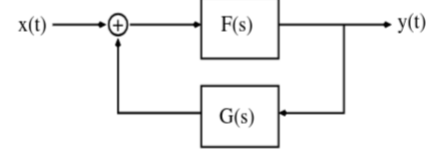
\includegraphics[width=0.5\textwidth]{Images/feedback_system.png}
    \end{center}
\end{exercise}

Let $W(s)$ be the Laplace transform of the input to $F(s)$. 

Then 
\begin{align*}
    W(s) &= X(S) + G(s) Y(s)\\
    Y(s) &= F(s) W(s)\\
    &= F(s) \left[X(s) + G(s) Y(s)\right]\\
    H(s) &= \frac{Y(s)}{X(s)}\\ 
    &= \frac{F(s)\left[X(s) + G(s) Y(s)\right] }{X(s)}\\ 
    &= F(s) \left[1 + G(s) H(s)\right]\\ 
\end{align*}
so 
\begin{align*}
    H(s) - F(s) G(s) H(s) &= F(s)\\
    H(s) \left[1 - F(s) G(s)\right] &= F(s)\\
    \implies H(s) &= \frac{F(s)}{1 - F(s) G(s)}
\end{align*}

\section{Quizlette 1}

\begin{exercise}
    \textbf{Exercise:} Sketch $s_1(t) = \delta(t - a)$ and $s_2(t) = \delta(a - t)$. What are the respective outputs if $s_1(t)$ and $s_2(t)$ are applied to the input of a linear time invariant system with impulse response $h(t)$?
\end{exercise}

\begin{center}
\begin{tikzpicture}
    \draw (0, 0) -- (3, 0); 
    \draw (0.5, 0) -- ++(0, 2); 
    \draw[blue, ->] (2, 0) -- ++(0, 1) node[above right] {$\delta(t- a) = \delta (a - t)$}; 
    \node[below] at (2, 0) {$a$};
\end{tikzpicture}
\end{center}

\emph{Recall:} the impulse response satisfies 
\begin{align*}
    \int h(\tau) \delta(t - a - \tau)\; d\tau &= h(t - a)\\ 
    \int h(\tau) \delta(a - t - \tau)\; d\tau &= \int h(\tau) \delta(t - a - \tau)\; d\tau \\ 
    &= h(t - a)
\end{align*}

\begin{exercise}
    \textbf{Exercise:} the impulse response of a system is $e^{-t}u(t)$. What is the system output if the input is $e^{-2t}u(t)$? Show your work
\end{exercise}

The output of a linear system if the convolution of the input with the impulse response. 

\begin{align*}
    y(t) &= e^{-t}u(t) \star e^{-2t}u(t)\\ 
    &= \int e^{-\tau}u(\tau) \cdot e^{-2(t- \tau)} u(t - \tau)\; d\tau \\ 
    &= \int_0^t e^{-\tau} e^{-2(t - \tau)}\; d\tau \\ 
    &= e^{-2t} \int_0^t e^{\tau}\; d\tau \\
    &= e^{-t} - e^{-2t} 
\end{align*}

\begin{exercise}
    \textbf{Exercise:} Suppose
    \[x(t) = \left(\frac{\sin 2\pi t}{\pi t}\right)^2 \]
    What is $X(f)$?
\end{exercise}

We know that 
\[R = \F\left(\frac{\sin 2\pi t}{\pi t}\right) = \frac{1}{2j\, \pi t} [\delta (f - 1) + \delta(f + 1)]\]
so 
\begin{align*}
    \F(R^2) &= R\star R\\ 
    &= \int R(\tau) R(f - \tau)\; d\tau\\
    &= \int \frac{1}{2j\, \pi \tau} [\delta(\tau - 1) + \delta(\tau + 1)] \cdot \frac{1}{2j\, \pi (f - \tau)} [\delta(f - \tau - 1) + \delta(f - \tau + 1)]\; d\tau\\
    &= -\frac{1}{(2\pi)^2} \int \frac{1}{\tau (f - \tau)} [\delta(\tau - 1) + \delta(\tau + 1)] [\delta(f - \tau - 1) + \delta(f - \tau + 1)]\; d\tau
\end{align*}


\begin{exercise}
    \textbf{Exercise:} Suppose $y(t) = x(t) \cos 2\pi f_0 t$. Is the system $y(t) = L[x(t)]$ linear? Is it time-invariant? 
\end{exercise}

\begin{align*}
    L[a_1 x_1(t) + a_2 x_2(t)] &= (a_1 x_1(t) + a_2 x_2(t)) \cos 2\pi f_0 t\\ 
    &= a_1 x_1(t) \cos 2\pi f_0 t + a_2 x_2(t) \cos 2\pi f_0 t\\
    &= a_1 L[x_1(t)] + a_2 L[x_2(t)]
\end{align*}
So linear. 

Now, time-invariance:
\begin{align*}
    L[x(t - t_0)] &= x(t - t_0) \cos 2\pi f_0 t\\ 
    &\neq y(t - t_0) = x(t - t_0) \cos 2\pi f_0 (t - t_0)
\end{align*}
so not time-invariant.
\chapter{Modulation}

Consider a simple modulation and demodulation scheme:
\begin{center}
\begin{tikzpicture}

    \node[blue] at (0.5, 0) {$m(t)$};

    \begin{axis}[
        at={(-1cm,-2.5cm)},
        width=0.2\textwidth,
        axis lines=middle,
        no markers,
        xtick=\empty,
        ytick=\empty,
        clip=false,
        xlabel={},
        ylabel={},
        domain=0.2:1.8,
        ymin=-1, ymax=3,
        xmin= -1, xmax=2,
        view = {0}{90}
    ]
        \addplot[blue] {(x-1)^2+1};
    \end{axis}

    \draw[->] (1, 0) -- ++(1, 0); 
    \draw (2.5, 0) circle (10pt) node {$\times$};
    \draw[<-] (2.5, -0.5) -- ++(0, -1.5) node[below] {$\cos 2\pi f_c t$};
    \draw (2.5, 0.5) -- ++(0, 1) node {\rotatebox{180}{\scalebox{2}{$\triangle$}}};
    \draw[dashed] (3, 1.5) -- ++(0.5, 0) node[right, blue] {$m(t) \cos 2\pi f_c t$};

    \begin{axis}[
        at={(3.5cm,-1cm)},
        width=0.2\textwidth,
        axis lines=middle,
        no markers,
        xtick=\empty,
        ytick=\empty,
        clip=false,
        xlabel={},
        ylabel={},
        domain=0.2:1.8,
        ymin=-3, ymax=3,
        xmin= -1, xmax=2,
        view = {0}{90}
    ]
        \addplot[blue, name path=p1] {(x-1)^2+1};
        \addplot[blue, name path=p2] {-(x-1)^2-1};
        \addplot[fill=blue, fill opacity=0.1] fill between[of=p1 and p2];

    \end{axis}

    \draw[dashed] (6.5, 1.5) -- ++(0.5, 0);
    \draw (7.5, 1.5) node {\rotatebox{180}{\scalebox{2}{$\triangle$}}} -- ++(0, -1);
    \draw (7.5, 0) circle (10pt) node {$\times$};
    \draw[<-] (7.5, -0.5) -- ++(0, -1.5) node[below] {$\cos 2\pi f_c t$};
    \draw[->] (8, 0) -- ++(0.5, 0) node[right, blue] {\scalebox{1.3}{$\begin{subarray}{l}
        m(t)\cos^2 2\pi f_c t\\ 
        =\frac{m(t)}{2} + \frac{m(t)\cos 2\pi f_c t}{2}
    \end{subarray}$}};

    \draw[->] (12.5, 0) -- ++(0.5, 0);
    \draw (13.5, -1.3) rectangle ++(2, 2.5) node[midway, yshift=0.7cm] {LPF};
    \draw[->] (16, 0) -- ++(0.5, 0) node[right, blue] {$\frac{m(t)}{2}$};

    \begin{axis}[
        at={(13.75cm,-1cm)},
        width=0.15\textwidth,
        axis lines=middle,
        no markers,
        xtick=\empty,
        ytick=\empty,
        clip=false,
        xlabel={},
        ylabel={},
        domain=0.2:1.8,
        ymin=-1, ymax=2,
        xmin= -2, xmax=2,
        view = {0}{90}
    ]
        \addplot[blue] coordinates {(-1, 0) (-1, 1) (1, 1) (1, 0)};
    \end{axis}
\end{tikzpicture}
\end{center}

for $m(t)$ a message and $f_c$ a carrier frequency ($f_c \gg B$, the bandwidth of $m(t)$) which transmits the message better since it is higher frequency.

What exactly is happening here? Let's look in the frequency domain:

\begin{enumerate}
    \item Modulation:
        
    \begin{center}
    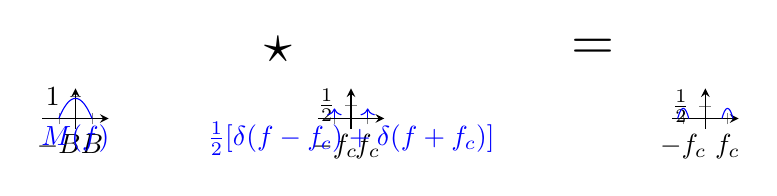
\begin{tikzpicture}
        \begin{axis}[
            at={(0cm,0cm)},
            width=0.2\textwidth,
            axis lines=middle,
            no markers,
            xtick={-1, 1},
            xticklabels={$-B$, $B$},
            ytick={2.2},
            yticklabels={1},
            clip=false,
            xlabel={},
            ylabel={},
            domain=-1:1,
            ymin=-1, ymax=3,
            xmin= -2, xmax=2,
            view = {0}{90}
        ]
            \addplot[blue] {-2*x^2+2};
            \node at (axis cs:0,-2) [blue] {$M(f)$};
        \end{axis}

        \node at (3, 1) {\scalebox{2}{$\star$}};

        \begin{axis}[
            at={(3.5cm,0cm)},
            width=0.2\textwidth,
            axis lines=middle,
            no markers,
            xtick={-1, 1},
            xticklabels={$-f_c$, $f_c$},
            ytick={1.3},
            yticklabels={$\frac{1}{2}$},
            clip=false,
            xlabel={},
            ylabel={},
            domain=-1:1,
            ymin=-1, ymax=3,
            xmin= -2, xmax=2,
            view = {0}{90}
        ]
        \draw[blue, ->] (-1, 0) -- (-1, 1);  
        \draw[blue, ->] (1, 0) -- (1, 1);  

        \node at (axis cs:0,-2) [blue] {$\frac{1}{2}[\delta(f-f_c) + \delta(f+f_c)]$};
        \end{axis}

        \node at (7, 1) {\scalebox{2}{$=$}};

        \begin{axis}[
            at={(8cm,0cm)},
            width=0.2\textwidth,
            axis lines=middle,
            no markers,
            xtick={-4, 4},
            xticklabels={$-f_c$, $f_c$},
            ytick={1.2},
            yticklabels={$\frac{1}{2}$},
            clip=false,
            xlabel={},
            ylabel={},
            ymin=-1, ymax=3,
            xmin= -6, xmax=6,
            view = {0}{90}
        ]
            \addplot[domain=-5:-3, blue] {-(x+4)^2+1};
            \addplot[domain=3:5, blue] {-(x-4)^2+1};

        \end{axis}    
    \end{tikzpicture}
    \end{center}

    Convolving with an impulse shifts the signal to be centered at the impulse!

    \item Demodulation:
    \begin{center}
    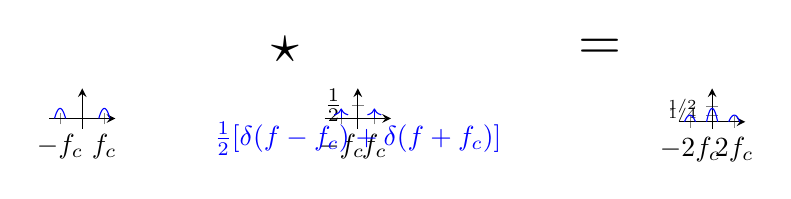
\begin{tikzpicture}
        \begin{axis}[
            at={(0cm,0cm)},
            width=0.2\textwidth,
            axis lines=middle,
            no markers,
            xtick={-4, 4},
            xticklabels={$-f_c$, $f_c$},
            ytick=\empty,
            clip=false,
            xlabel={},
            ylabel={},
            ymin=-1, ymax=3,
            xmin= -6, xmax=6,
            view = {0}{90}
        ]
            \addplot[domain=-5:-3, blue] {-(x+4)^2+1};
            \addplot[domain=3:5, blue] {-(x-4)^2+1};

        \end{axis}    

        \node at (3, 1) {\scalebox{2}{$\star$}};

        \begin{axis}[
            at={(3.5cm,0cm)},
            width=0.2\textwidth,
            axis lines=middle,
            no markers,
            xtick={-1, 1},
            xticklabels={$-f_c$, $f_c$},
            ytick={1.3},
            yticklabels={$\frac{1}{2}$},
            clip=false,
            xlabel={},
            ylabel={},
            domain=-1:1,
            ymin=-1, ymax=3,
            xmin= -2, xmax=2,
            view = {0}{90}
        ]
        \draw[blue, ->] (-1, 0) -- (-1, 1);  
        \draw[blue, ->] (1, 0) -- (1, 1);  

        \node at (axis cs:0,-2) [blue] {$\frac{1}{2}[\delta(f-f_c) + \delta(f+f_c)]$};
        \end{axis}

        \node at (7, 1) {\scalebox{2}{$=$}};

        \begin{axis}[
            at={(8cm,0cm)},
            width=0.2\textwidth,
            axis lines=middle,
            no markers,
            xtick={-4, 4},
            xticklabels={$-2f_c$, $2f_c$},
            ytick={1, 2.3},
            yticklabels={{\tiny 1/4}, {\tiny 1/2}},
            clip=false,
            xlabel={},
            ylabel={},
            ymin=-1, ymax=5,
            xmin= -6, xmax=6,
            view = {0}{90}
        ]
            \addplot[domain=-5:-3, blue] {-(x+4)^2+1};
            \addplot[domain=3:5, blue] {-(x-4)^2+1};
            \addplot[domain=-1:1, blue] {-2*x^2+2};
        \end{axis}    
    \end{tikzpicture}
    \end{center}

    (spread a copy of the signal around $-f_c$ and $f_c$ so that the interference terms reinforce each other at the baseband)

    \item Filtering:

    \begin{center}
    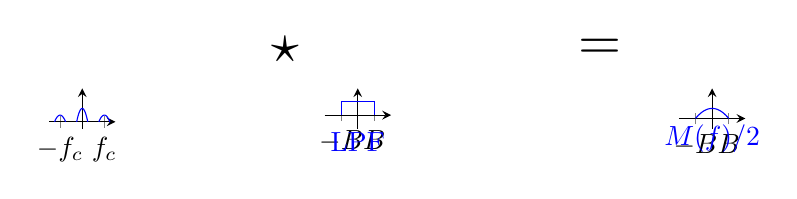
\begin{tikzpicture}
        \begin{axis}[
            at={(0cm,0cm)},
            width=0.2\textwidth,
            axis lines=middle,
            no markers,
            xtick={-4, 4},
            xticklabels={$-f_c$, $f_c$},
            ytick=\empty,
            clip=false,
            xlabel={},
            ylabel={},
            ymin=-1, ymax=5,
            xmin= -6, xmax=6,
            view = {0}{90}
        ]
            \addplot[domain=-5:-3, blue] {-(x+4)^2+1};
            \addplot[domain=3:5, blue] {-(x-4)^2+1};
            \addplot[domain=-1:1, blue] {-2*x^2+2};
        \end{axis}  

        \node at (3, 1) {\scalebox{2}{$\star$}};

        \begin{axis}[
            at={(3.5cm,0cm)},
            width=0.2\textwidth,
            axis lines=middle,
            no markers,
            xtick={-2, 2},
            xticklabels={$-B$, $B$},
            ytick=\empty,
            clip=false,
            xlabel={},
            ylabel={},
            ymin=-1, ymax=2,
            xmin= -4, xmax=4,
            view = {0}{90}
        ]
            \addplot[blue] coordinates {(-2, 0) (-2, 1) (2, 1) (2, 0)};
            \node at (axis cs:0,-2) [blue] {LPF};
        \end{axis}

        \node at (7, 1) {\scalebox{2}{$=$}};

        \begin{axis}[
            at={(8cm,0cm)},
            width=0.2\textwidth,
            axis lines=middle,
            no markers,
            xtick={-1, 1},
            xticklabels={$-B$, $B$},
            ytick=\empty,
            clip=false,
            xlabel={},
            ylabel={},
            domain=-1:1,
            ymin=-1, ymax=3,
            xmin= -2, xmax=2,
            view = {0}{90}
        ]
            \addplot[blue] {-x^2+1};
            \node at (axis cs:0,-2) [blue] {$M(f)/2$};
        \end{axis}

    \end{tikzpicture}
    \end{center}
\end{enumerate}

\section{Feb 3}

\tbf{Coherent AM:} Synchronous modulation; Modulate with $\cos 2\pi f_c t$ and demodulate with the same signal.

Recall in our demodulation step we multiplied by $\cos 2\pi f_c t$ again. What if we made a mistake and used $\sin(2\pi f_c t)$ instead? 

    \begin{center}
    \begin{tikzpicture}
        \begin{axis}[
            at={(0cm,0cm)},
            width=0.2\textwidth,
            axis lines=middle,
            no markers,
            xtick={-4, 4},
            xticklabels={$-f_c$, $f_c$},
            ytick=\empty,
            clip=false,
            xlabel={},
            ylabel={},
            ymin=-1, ymax=3,
            xmin= -6, xmax=6,
            view = {0}{90}
        ]
            \addplot[domain=-5:-3, blue] {-(x+4)^2+1};
            \addplot[domain=3:5, blue] {-(x-4)^2+1};

        \end{axis}    

        \node at (3, 1) {\scalebox{2}{$\star$}};

        \begin{axis}[
            at={(3.5cm,0cm)},
            width=0.2\textwidth,
            axis lines=middle,
            no markers,
            xtick={-1, 1},
            xticklabels={$-f_c$, $f_c$},
            ytick={1.3},
            yticklabels={$\frac{1}{2}$},
            clip=false,
            xlabel={},
            ylabel={},
            domain=-1:1,
            ymin=-2, ymax=3,
            xmin= -2, xmax=2,
            view = {0}{90}
        ]
        \draw[blue, ->] (-1, 0) -- (-1, -1);  
        \draw[blue, ->] (1, 0) -- (1, 1);  

        \node at (axis cs:0,-4) [blue] {$\begin{subarray}{c}
            \F(\sin 2\pi f_c t) = \\ 
            \frac{1}{2j}[\delta(f-f_c) - \delta(f+f_c)]
            
        \end{subarray}$};
        \end{axis}

        \node at (7, 1) {\scalebox{2}{$=$}};

        \begin{axis}[
            at={(8cm,0cm)},
            width=0.2\textwidth,
            axis lines=middle,
            no markers,
            xtick={-4, 4},
            ytick=\empty,
            xticklabels={$-2f_c$, $2f_c$},
            clip=false,
            xlabel={},
            ylabel={},
            ymin=-3, ymax=5,
            xmin= -6, xmax=6,
            view = {0}{90}
        ]
            \addplot[domain=-5:-3, red] {(x+4)^2-1};
            \addplot[domain=-1:1, red] {x^2-1};

            \addplot[domain=3:5, blue] {-(x-4)^2+1};
            \addplot[domain=-1:1, blue] {-x^2+1};
        \end{axis}    
    \end{tikzpicture}
    \end{center}

    So the signals cancel around the baseband and we get no message after filtering!

    How could we recover if we made this mistake? 

    Let's try broadcasting two messages $m_1(t) \cos 2\pi f_c t$ and $m_2(t) \sin 2\pi f_c t$ simultaneously.

    The received signal is $(s_1(t) + s_2(t))$. If we demodulate by $\cos 2\pi f_c t$ on one rail and $\sin 2\pi f_c t$ on the other rail and filter, we get two separate messages back, $m_1(t)/2$ and $m_2(t)/2$ respectively! 

    \begin{center}
    \begin{tikzpicture}
       
    \node at (0.5, 0) [blue] {$m_1(t)$};
    \draw[->] (1, 0) -- ++(1, 0); 
    \draw (2.5, 0) circle (10pt) node {$\times$};
    \draw[<-] (2.5, -0.5) -- ++(0, -0.5) node[below] {$\cos 2\pi f_c t$};
    \draw (2.5, 0.5) -- ++(0, 1) node {\rotatebox{180}{\scalebox{2}{$\triangle$}}};
    \draw[dashed] (3, 1.5) -- ++(0.5, 0) node[right, blue] {$s_1(t)$};

    \node at (0.5, -4) [blue] {$m_2(t)$};
    \draw[->] (1, -4) -- ++(1, 0); 
    \draw (2.5, -4) circle (10pt) node {$\times$};
    \draw[<-] (2.5, -4.5) -- ++(0, -0.5) node[below] {$\sin 2\pi f_c t$};
    \draw (2.5, -3.5) -- ++(0, 1) node {\rotatebox{180}{\scalebox{2}{$\triangle$}}};
    \draw[dashed] (3, -2.5) -- ++(0.5, 0) node[right, blue] {$s_2(t)$};

    \draw[dashed] (7.5, 0)  node[left, blue] {$s_1(t) + s_2(t)$} -- ++(0.5, 0);
    \draw (8.5, 0) node {\rotatebox{180}{\scalebox{2}{$\triangle$}}} -- ++(0, -4);

    \draw[->] (8.5, -1) -- ++(1, 0); 
    \draw (10, -1) circle (10pt) node {$\times$};
    \draw[<-] (10, -1.5) -- ++(0, -0.5) node[below] {$\cos 2\pi f_c t$};
    \draw (10.5, -1) -- ++(1, 0) node[right, draw, rectangle] {LPF};
    \draw (12.75, -1) -- ++(1, 0) node[right, blue] {$\frac{m_1(t)}{2}$};

    \draw[->] (8.5, -4) -- ++(1, 0); 
    \draw (10, -4) circle (10pt) node {$\times$};
    \draw[<-] (10, -4.5) -- ++(0, -0.5) node[below] {$\sin 2\pi f_c t$};
    \draw (10.5, -4) -- ++(1, 0) node[right, draw, rectangle] {LPF};
    \draw (12.75, -4) -- ++(1, 0) node[right, blue] {$\frac{m_2(t)}{2}$};

    \end{tikzpicture}
    \end{center}

    \tbf{Single sideband modulation:} Let $m(t)$ be a real signal with Fourier transform $M(f)$. We know 
    \begin{align*}
        M(f) &= \int m(t) e^{-j\; 2\pi ft}\; dt\\ 
        M^*(f) &= \int m(t) e^{-j\; 2\pi (-f)t}\; dt = M(-f)
    \end{align*}
    (i.e. the real part is even and the imaginary part is odd)

    In particular, this means we can send less information by sending only the positive frequencies or only the negative frequencies and reconstructing the other half using the even/odd properties.

    \begin{enumerate}
        \item Modulate $m(t)$ by $\cos 2\pi f_c t$ to shift the spectrum to be centered at $\pm f_c$.
        
        \begin{center}
        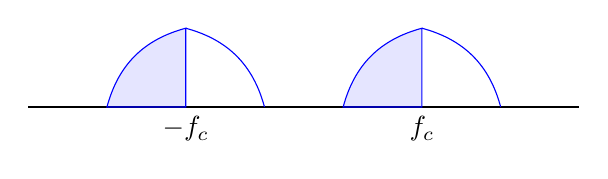
\begin{tikzpicture}
            \draw (0, 0) -- (7, 0);

            \draw[fill, blue, fill opacity=0.1] (1, 0) to[bend left] ++(1, 1) -- ++(0, -1) -- ++(-1, 0) -- cycle;
            \draw[blue]  (2, 1) to[bend left] ++(1, -1);
            \node[below] at (2, 0) {$-f_c$};


            \draw[fill, blue, fill opacity=0.1] (4, 0) to[bend left] ++(1, 1) -- ++(0, -1) -- ++(-1, 0) -- cycle;
            \draw[blue]  (5, 1) to[bend left] ++(1, -1);
            \node[below] at (5, 0) {$f_c$};
        \end{tikzpicture}
        \end{center}

        \item Filter 
        \begin{center}
        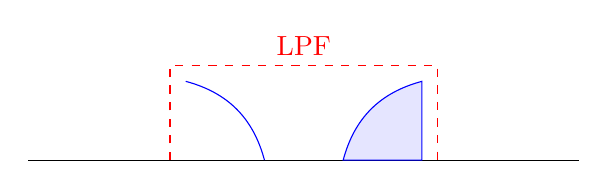
\begin{tikzpicture}
                \draw (0, 0) -- (7, 0);

                \draw[blue]  (2, 1) to[bend left] ++(1, -1);
                \draw[fill, blue, fill opacity=0.1] (4, 0) to[bend left] ++(1, 1) -- ++(0, -1) -- ++(-1, 0) -- cycle;

                \draw[dashed, red] (1.8, 0) -- ++(0, 1.2) -- node[midway, above] {LPF} ++(3.4, 0) -- ++(0, -1.2);
            \end{tikzpicture}
            \end{center}

        \item Transmit
        \item Demodulate by multiplying by $\cos 2\pi f_c t$ again.
        \begin{center}
        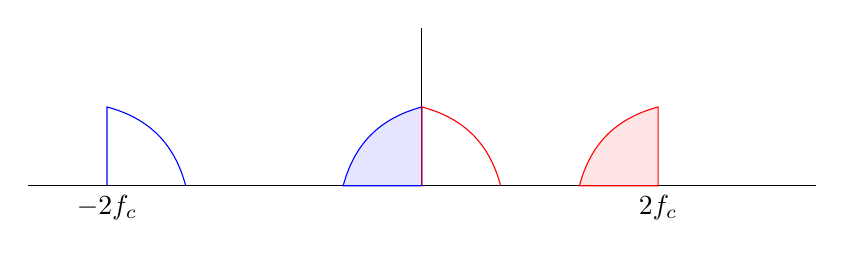
\begin{tikzpicture}
            \draw (0, 0) -- (10, 0);
            \draw (5, 0) -- ++(0, 2);

            \draw[blue] (1, 0) -- (1, 1) to[bend left] ++(1, -1); 
            
            \draw[fill, blue, fill opacity=0.1] (4, 0) to[bend left] ++(1, 1) -- ++(0, -1) -- ++(-1, 0) -- cycle;
            \draw[red] (5, 0) -- ++(0, 1) to[bend left] ++(1, -1); 
            \draw[fill, red, fill opacity=0.1] (7, 0) to[bend left] ++(1, 1) -- ++(0, -1) -- ++(-1, 0) -- cycle;

            \node[below] at (1, 0) {$-2f_c$};
            \node[below] at (8, 0) {$2f_c$};
        \end{tikzpicture}
        \end{center}

        \item LPF again to recover the full signal using half the bandwidth! 
    \end{enumerate}

    \tbf{Frequency Division Multiplexing:}

    Define two signals $m_1(t)$ and $m_2(t)$. 

    \begin{center}
        \begin{multicols}{2}
            \begin{tikzpicture}
            \draw (0, 0) -- (4, 0) node[right] {$f$};
            \draw (2, 2) -- ++(0, -2) node[below] {$M_1(f)$};
            \draw[blue] (1, 0) to[bend left] ++(1, 1) to[bend left] ++(1, -1);
        \end{tikzpicture}

        \begin{tikzpicture}
            \draw (0, 0) -- (4, 0) node[right] {$f$};
            \draw (2, 2) -- ++(0, -2) node[below] {$M_2(f)$};
            \draw[blue] (1, 0) -- ++(1, 1) -- ++(1, -1);
        \end{tikzpicture}
        \end{multicols}
    \end{center}


    \begin{center}
    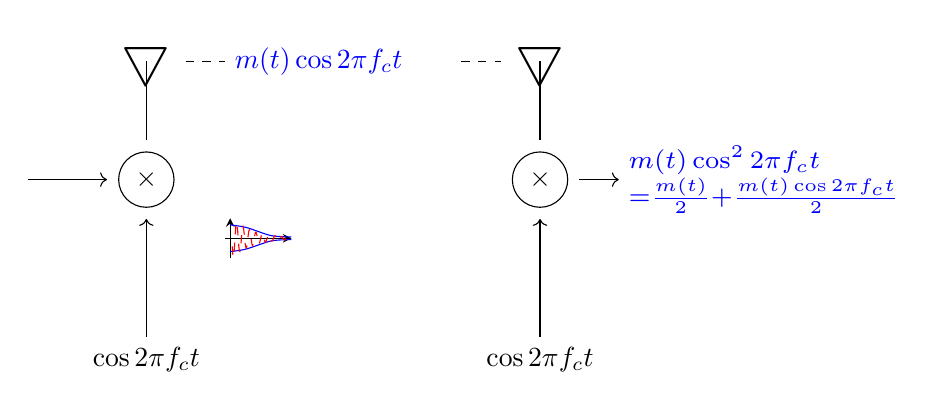
\begin{tikzpicture}
        \draw[->] (1, 0) -- ++(1, 0); 
        \draw (2.5, 0) circle (10pt) node {$\times$};
        \draw[<-] (2.5, -0.5) -- ++(0, -1.5) node[below] {$\cos 2\pi f_c t$};
        \draw (2.5, 0.5) -- ++(0, 1) node {\rotatebox{180}{\scalebox{2}{$\triangle$}}};
        \draw[dashed] (3, 1.5) -- ++(0.5, 0) node[right, blue] {$m(t) \cos 2\pi f_c t$};

        \draw[dashed] (6.5, 1.5) -- ++(0.5, 0);
        \draw (7.5, 1.5) node {\rotatebox{180}{\scalebox{2}{$\triangle$}}} -- ++(0, -1);
        \draw (7.5, 0) circle (10pt) node {$\times$};
        \draw[<-] (7.5, -0.5) -- ++(0, -1.5) node[below] {$\cos 2\pi f_c t$};
        \draw[->] (8, 0) -- ++(0.5, 0) node[right, blue] {\scalebox{1.3}{$\begin{subarray}{l}
            m(t)\cos^2 2\pi f_c t\\ 
            =\frac{m(t)}{2} + \frac{m(t)\cos 2\pi f_c t}{2}
        \end{subarray}$}};

  
        \begin{axis}[
            width=0.2\textwidth,
            at={(3.5cm,-1cm)},
            axis lines=middle,
            no markers,
            xtick=\empty,
            ytick=\empty,
            clip=false,
            xlabel={},
            ylabel={},
            domain=-2:2,
            ymin=-1.5, ymax=1.5,
            xmin= -0.25, xmax=3,
            view = {0}{90}
        ]

        \addplot[smooth, blue] coordinates {(0, 1) (0.8, 0.8) (2, 0.2) (3, 0.1)};
        \addplot[smooth, blue] coordinates {(0, -1) (0.8, -0.8) (2, -0.2) (3, -0.1)};

        \addplot[red, dashed, domain=0.1:3, samples=100] {0.6*exp(1-x) * cos(20*deg(x))}; 

        
        \end{axis}
    
    \end{tikzpicture}
    \end{center}    

    Though we could also blow up in time and rectify the transmitted wave 

   \begin{center}
   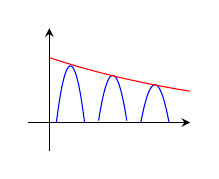
\begin{tikzpicture}
   \begin{axis}[
       width=0.3\textwidth,
       axis lines=middle,
       no markers,
       xtick=\empty,
       ytick=\empty,
       clip=false,
       xlabel={},
       ylabel={},
       domain=-2:2,
       ymin=-0.3, ymax=1,
       xmin= -0.3, xmax=2,
       samples=100,
       view = {0}{90}
   ]
       \addplot[blue, domain=0.1:0.5] {-15*(x-0.3)^2 + 0.6};
       \addplot[blue, domain=0.7:1.1] {-12*(x-0.9)^2 + 0.5};
       \addplot[blue, domain=1.3:1.7] {-10*(x-1.5)^2 + 0.4};
       \addplot[red, domain=0:2] {0.688883*0.69359^x};


   \end{axis}
   \end{tikzpicture}
   \end{center}

   so we can recover the envelope (all the information is in the amplitude of the envelope), for example using this circuit:

   \begin{center}
    \begin{circuitikz}[american voltages]
         \node at (-0.5, 0) {$r(t)$}; 
         \draw (0, 0) to[diode] (2, 0)
             to[resistor] (2, -2)
             -- (2, -2) node[below, ground] {} ;
 
         \draw (2, 0) -- ++(2, 0) to[capacitor] ++(0, -2) -- ++(-2, 0);
         \draw (4, 0) -- ++(1, 0) node[right] {$\hat m(t)$};
 
    \end{circuitikz}
   \end{center}


\tbf{Motivating FM:}
\[r(t) = \sin\left(2\pi f_c t + \int_{-\infty}^t m(\tau) d\tau \right) \]

Where is the information here? In the integral. 

What does it look like? First, we know it has constant amplitude (``modulus 1'').

Define the \emph{instantaneous frequency} 
\[\omega(t) = \frac{d}{dt} \Theta(t) = 2\pi f_0 = \omega_0\]
for $\Theta(t) = 2\pi f_0 t$ the \emph{instantaneous phase} of the signal.

Now let's try differentiating:

\begin{align*}
    \frac{d}{dt} r(t) &= (2\pi f_c + m(t)) \cos \left(2\pi f_c t + \int_{-\infty}^t m(\tau)\; d\tau\right) 
\end{align*}

\section{Feb 5}
\subsection{AM Review}

\tbf{Coherent Modulation:} Modulate and demodulate by multiplying with the same carrier signal (traditionally $\cos 2\pi f_c t$). Recover $\alpha m(t)$ after low-pass filtering.

\tbf{Large Carrier (LC) Modulation:} Transmit the message $(m(t) + A) \cos 2\pi f_c t$ with $A \geq \max_t \abs{m(t)}$ (though this is a bit overkill to ensure $m(t) + A \geq 0$). Receive with an envelope detector, LPF, and very low HPF (to remove the DC offset $A$).

Why do we need to make sure the message is always positive? To an envelope detector, there is no difference between $m(t) + A$ and $\abs{m(t) + A}$. If $m(t) + A$ goes negative, the envelope detector will just flip it positive and distort the message.

\begin{center}
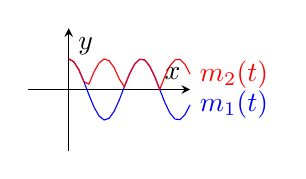
\begin{tikzpicture}
\begin{axis}[
    width=0.3\textwidth,
    axis lines=middle,
    no markers,
    xtick=\empty,
    ytick=\empty,
    clip=false,
    xlabel={$x$},
    ylabel={$y$},
    ymin=-2, ymax=2,
    xmin= -2, xmax=6,
    view = {0}{90}
]
    \addplot[blue, domain=0:6] {cos(100*x)} node[right] {$m_1(t)$};
    \addplot[red, domain=0:6] {abs(cos(100*x))} node[right] {$m_2(t)$};
\end{axis}

\end{tikzpicture}
\end{center}

What does the transmitted signal look like in the frequency domain? 

    \begin{center}
    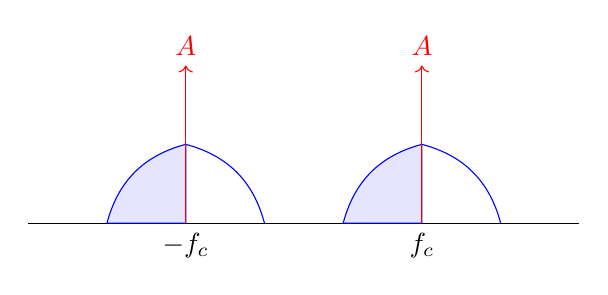
\begin{tikzpicture}
        \draw (0, 0) -- (7, 0);

        \draw[fill, blue, fill opacity=0.1] (1, 0) to[bend left] ++(1, 1) -- ++(0, -1) -- ++(-1, 0) -- cycle;
        \draw[blue]  (2, 1) to[bend left] ++(1, -1);
        \node[below] at (2, 0) {$-f_c$};


        \draw[fill, blue, fill opacity=0.1] (4, 0) to[bend left] ++(1, 1) -- ++(0, -1) -- ++(-1, 0) -- cycle;
        \draw[blue]  (5, 1) to[bend left] ++(1, -1);
        \node[below] at (5, 0) {$f_c$};

        \draw[->, red] (2, 0) -- ++(0, 2) node[above] {$A$};
        \draw[->, red] (5, 0) -- ++(0, 2) node[above] {$A$};


    \end{tikzpicture}
    \end{center}


Exactly the same as coherent AM but with impulses added at the message frequencies. 

\tbf{Single Sideband (SSB) Modulation:} can be coherent or incoherent. Before transmitting apply an LPF so we use half the bandwidth. This takes advantage of the fact that $M(-f) = M^*(f)$. For lower sideband, we can invert the initial filter and pack a second message into the other (filtered) part of the spectrum. 


\begin{center}
\begin{tikzpicture}
    \node at (0, 0) [red] {$m_1(t)$};
    \draw[->, shorten >= 5pt, shorten <= 5pt] (0.5, 0) --  ++(1, 0) node[right, draw, rectangle] {\begin{tabular}{c}
        U\\ 
        SSB 
    \end{tabular}};
    \draw (2.3, 0.8) -- ++(0, 1) node {\scalebox{2}{\rotatebox{180}{$\triangle$}}}; 

    \node at (0, -4) [blue] {$m_2(t)$};
    \draw[->, shorten >= 5pt, shorten <= 5pt] (0.5, -4) --  ++(1, 0) node[right, draw, rectangle] {\begin{tabular}{c}
        L\\ 
        SSB 
    \end{tabular}};
    \draw (2.3, -3.2) -- ++(0, 1) node {\scalebox{2}{\rotatebox{180}{$\triangle$}}}; 

    \draw (-1, 1) -- ++(2, 0);
    \draw (0, 1) -- ++(0, 1);
    \draw[red, decoration=coil, decorate] (-0.7, 1.5) -- ++(1.4, 0);
    \draw[red] (-0.7, 1) -- ++(0, 0.5);
    \draw[red] (0.7, 1) -- ++(0, 0.5);

    \draw (-1, -3) -- ++(2, 0);
    \draw (0, -3) -- ++(0, 1);
    \draw[blue] (-0.5, -3) arc (180:0:0.5 and 0.8);

    \draw (4, 0) -- ++(3, 0);
    \draw (5.5, 0) -- ++(0, 1);
    \draw[red, decoration=coil, decorate] (4.1, 0.5) -- (4.8, 0.5);
    \draw[red] (4.1, 0.5) -- ++(0, -0.5);
    \draw[red] (4.8, 0.5) -- ++(0, -0.5) node[below, black] {$-f_c$} ;
    
    \draw[red, decoration=coil, decorate] (6.2, 0.5) -- (6.9, 0.5);
    \draw[red] (6.2, 0.5) -- ++(0, -0.5) node[below, black] {$f_c$};
    \draw[red] (6.9, 0.5) -- ++(0, -0.5) ;    
    \draw[red] (-0.7, 1) -- ++(0, 0.5);
    \draw[red] (0.7, 1) -- ++(0, 0.5);

    \draw (4, -4) -- ++(3, 0);
    \draw (5.5, -4) -- ++(0, 1);
    \draw[blue] (4.8, -4) node[black, below] {$-f_c$} -- ++(0, 0.5) to[bend left] ++(0.5, -0.5);
    \draw[blue] (6.2, -4) node[black, below] {$-f_c$} -- ++(0, 0.5) to[bend right] ++(-0.5, -0.5);
\end{tikzpicture}
\end{center}

\emph{What happens if we modulated with a square wave instead of a cosine wave?} The square wave can be expressed as a Fourier series of cosines at odd harmonics of the fundamental frequency. In the frequency domain, this looks just like the coherent AM case but with copies of the message at all the harmonics (impulses at $f_c, 3f_c, 5f_c, \ldots$).

\subsection{FM} 

Let 
\[r(t) = \sin (\Theta(t)) = \sin\left(2\pi f_c t + \beta\int_{-\infty}^t m(\tau) \; d\tau\right)\]

This is a constant amplitude signal with changing frequency. 

\tbf{Instantaneous Frequency:}
\[\frac{d\Theta(t)}{dt} = \omega(t) \]

What happens if we differentiate $r(t)$?
\[    \frac{dr}{dt} = (2\pi f_c + \beta m(t)) \cos\left(2\pi f_c t + \beta\int_{-\infty}^t m(\tau)\; d\tau\right) 
\] 

Since $f_c \gg m(t)$ and we assume $\beta$ is relatively small (hence $\beta \int_{-\infty}^t m(\tau)\; d\tau \lll 1$) we can just throw this into an envelope detector and HPF (get rid of the DC term) to recover $\beta m(t)$ approximately.

\begin{center}
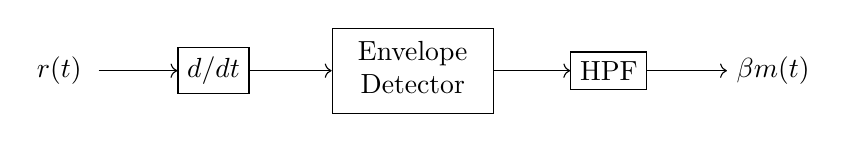
\begin{tikzpicture}
    \node at (0, 0) {$r(t)$}; 
    \draw[->] (0.5, 0) -- ++(1, 0) node[right, draw, rectangle] (A) {$d/dt$};
    \draw[->] (A) -- ++(1.5, 0) node[right, draw, rectangle] (B) {\begin{tabular}{c}
        Envelope \\ 
        Detector
    \end{tabular}}; 
    \draw[->] (B) -- ++(2, 0) node[right, draw, rectangle] (C) {HPF};
    \draw[->] (C) -- ++(1.5, 0) node[right] {$\beta m(t)$};
\end{tikzpicture}
\end{center}

In particular, 
\begin{align*}
    r(t) &= \sin (2\pi f_c t) \cos (\beta \Theta(t)) + \cos (2\pi f_c t) \sin (\beta \Theta(t))\\ 
    &\approx (\cos 2\pi f_c t) \left(\beta \int_{-\infty}^t m(\tau)\; d\tau\right) + \sin 2\pi f_c t \qquad (\sin x = x)
\end{align*}

\section{Feb 10 - Quiz 1 Review}

\emph{What is a linear system? 
}\[L[au + bv] = aL[u] + bL[v], \quad a, b \in \R\]

\emph{Is $y = ax + b$ ($a, b \neq 0$) linear? }
No. It doesn't satisfy scaling: 
\[y = a(cx) + b \neq c(ax + b)\]

\emph{What is a linear time-invariant (LTI) system?
}
\[y(t) = L[x(t)] \implies y(t - t_0) = L{x(t - t_0)}\]

\emph{What is a delta function?}
\begin{enumerate}
    \item $\int \delta(t)\; dt = 1$
    \item $\delta(t) = 0$ for $t \neq 0$
    \item $\int f(t) \delta(t - t_0)\; dt = f(t_0)$ (sifting)
\end{enumerate}

\tbf{Transfer function:} $H(f) = \F(h(t))$ where $h(t)$ is the \tbf{impulse response} of the system.

\begin{center}
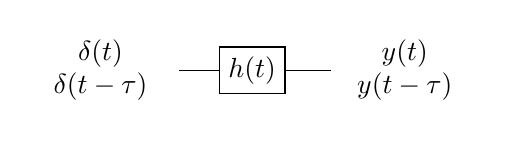
\begin{tikzpicture}
    \node at (0, 0) {\begin{tabular}{c}
        $\delta(t)$\\ 
        $\delta(t - \tau)$ 
    \end{tabular}};
    \draw (1, 0) -- ++(0.5, 0) node[right, draw, rectangle] (A) {$h(t)$};
    \draw (A) -- ++(1, 0) node[right] {\begin{tabular}{c}
        $y(t)$\\ 
        $y(t - \tau)$
    \end{tabular}};
\end{tikzpicture}
\end{center}
where the box represents a \tbf{convolution}:
\[y(t) = (x * h)(t) = \int_{-\infty}^\infty x(\tau) h(t - \tau) \; d\tau
\]
(in fact, in the frequency domain, this operation is defined by $Y(f) = X(f) H(f)$)

\emph{Fourier Transform:} 
\[\F[x(t)] = \int x(t)e^{-j\; 2\pi ft} \; dt = X(f)\]

\emph{Inverse Fourier:}
\[\F^{-1}[X(f)] = \int X(f) e^{j \; 2\pi ft} \; df = x(t)\]

\emph{Standard Fourier pairs:}
\begin{enumerate}
    \item $\F[\delta(t)] = 1$
    \item $\F[e^{-j\; 2\pi f_0 t}] = \delta(f + f_0)$
    \item $\F[\delta(t- t_0)] = e^{-j\; 2\pi f t_0}$
    \item $\F[\cos 2\pi f_0 t] = \frac{1}{2}[\delta(f + f_0) + \delta(f - f_0)]$
    \item $\F[\sin 2\pi f_0 t] = \frac{1}{2j}[\delta(f + f_0) - \delta(f - f_0)]$
    \item $\F[\ind_{x\in [-T/2, T/2]}] = \text{sinc}(2\pi Tf)$
\end{enumerate}

\emph{Fourier Properties:}
\begin{enumerate}
    \item $\F[x(t - t_0)] = e^{j\; 2\pi f t_0} X(f)$
    \item $\F[ax(t)] = aX(f/a)$
    \item $\F[x'(t)] = X(f) \cdot j\; 2\pi f$
    \item $\F[\int_{-\infty}^t x(u)\; du] = \frac{X(f)}{j\; 2\pi f} + \frac{X(0)}{2} \delta(f)$
    \item $\int_{-\infty}^{\infty} \abs{x(t)}^2 = \int_{-\infty}^{\infty} \abs{X(f)}^2$ (Parseval's)
    \item $\F[X(t)] = x(-f)$  
\end{enumerate}

\emph{Useful tricks:}
\begin{enumerate}
    \item $\abs{X(f)}^2 = X(f) X^*(f) = X(f) X(-f)$
    \item $\cos(2\pi f t) = \frac{e^{j\; 2\pi f t} + e^{-j\; 2\pi f t}}{2}$
    \item $\sin(2\pi f t) = \frac{e^{j\; 2\pi f t} - e^{-j\; 2\pi f t}}{2j}$
    \item Fourier of odd function is purely imaginary, Fourier of even function is purely real.
    \item $\delta$ is an even function: $\delta(-t) = \delta(t)$
    \item $u(t) = \ind_{t \geq 0}(t)$ 
    \item $\sin(x + y) = \sin x \cos y + \cos x \sin y$
    \item $\cos(x + y) = \cos x \cos y - \sin x \sin y$
    \item $\sin^2 x = (1 - \cos 2 x)/2$
    \item $\cos^2 x = (1 + \cos 2x)/ 2$
    \item $\cos \theta(t) = \sum_{m=0}^{\infty} \frac{(\theta(t))^{2m}}{(2m)!}$
    \item $\sin \theta(t) = \sum_{m=0}^{\infty} (-1)^m \frac{(\theta(t))^{2m+1}}{(2m + 1)!}$
\end{enumerate}

\emph{Baseband:} unmodulated signal (i.e. the message signal).

\emph{Passband:} modulated signal (i.e. the transmitted signal).

\subsection{Modulation}

\emph{AM Coherent modulation:} $r(t) = m(t) \cos 2\pi f_c t$, demodulate with $\cos 2\pi f_c t$ and LPF to recover $m(t)/2$.

\emph{AM Large carrier:} $r(t) = (m(t) + A) \cos 2\pi f_c t$ ($A \gg m(t)$), demodulate with an envelope detector, LPF, and HPF to recover $m(t)$.

\emph{AM Single sideband:} $r(t) = m(t) \cos 2\pi f_c t$ with an LPF applied to $m(t)$ before modulation (takes advantage of symmetry from $M(-f) = M^*(f)$ to use half the bandwidth), demodulate with $\cos 2\pi f_c t$ and LPF to recover $m(t)/2$.

\emph{Frequency modulation:} $r(t) = \sin (2\pi f_c t + \beta \int_{-\infty}^t m(\tau)\; d\tau)$, demodulate by differentiating, envelope detecting, and HPF to recover $\beta m(t)$.

\emph{Phase modulation:} $r(t) = \sin (2\pi f_c t + \beta m(t))$ (filter and integrate)

\emph{How do you determine the bandwidth of an FM signal? What does it look like in the frequency domain? Hint: use linear system properties}

\section{Feb 19 - Sampling}

So far $m(t)$ has been a continuous-time signal. How do we represent it in the digital regime?

We assumed the spectrum of $m(t)$ is band-limited to $B$ Hz. How do we represent 
\[m(t) \to \{m_1, m_2, \dots\}\] 
a set of samples? (And especially a set of samples that we can use to reconstruct $m(t)$?)

\emph{Trick:} 
\[m(t) \lambda(t) = m(t) \sum_k \delta(t - kt)\] 

\begin{center}
\begin{tikzpicture}
    \draw (0, 0) -- (8, 0); 
    \draw (4, -0.5) -- ++(0, 1);
    \foreach \x in {0, 1, 2, 3, 4, 5, 6, 7} {
        \draw[->, blue] (\x, 0) -- (\x, 1.3*rand);
    }
\end{tikzpicture}
\end{center}

What is the spectrum of this sampled signal?
\begin{align*}
    M(f) \star \Lambda(f) &= M(f) \star \int e^{-j\; 2\pi ft} \sum_k \delta(t - kT)\; dt\\ 
    &= M(f) \star \sum_k e^{-j\; 2\pi fkT}\\
\end{align*}

Unfortunately, this tells us nothing. 

Instead, let's represent $\lambda$ via \tbf{Fourier series}:
\[\lambda(t) = \sum_{\ell = -\infty}^{\infty} \lambda_{\ell} e^{j\, \frac{2\pi}{T} \ell t}\]
where 
\[\lambda_{\ell} = \frac{1}{T} \int_{-T/2}^{T/2} \lambda(t) e^{-j\, \frac{2\pi}{T} \ell T} \; dt = \frac{1}{T}\]
(note that on $t \in [-T/2, T/2]$, $\lambda$ is a single impulse)

Hence, 
\[\lambda(t) = \frac{1}{T}\sum_{\ell} e^{j\; \frac{2\pi}{T} \ell t}\]
and using Fourier pairs, 
\[\Lambda(f) = \frac{1}{T} \sum_{\ell} \delta(f - \frac{\ell}{T})\]

\begin{center}
\begin{tikzpicture}
    \draw (-3, 0) -- (3, 0); 
    \draw (0, -0.5) -- ++(0, 2);
    \foreach \x in {-2, -1, 1, 2} {
        \draw[<-, blue] (\x, 1) -- (\x, 0) node[below] {$\frac{\x}{T}$};
    }
        \draw[->, blue] (0, 0) -- (0, 1) node[above right] {$\frac{1}{T}$};

\end{tikzpicture}
\end{center}

Hence, we can draw $M(f) \star \Lambda(f)$

% \begin{center}
% \begin{tikzpicture}
%     \draw (0, 0) -- (10, 0);

%     \foreach \x in {1, ... , 8} {
%         \draw (\x, 0) arc (90:270:0.5 and 1);
%     }
% \end{tikzpicture}
% \end{center}

and using an LPF brings back our signal. 

This also gives us the \tbf{Nyquist Criterion} 
\[\frac{1}{T} - B > B \implies \boxed{\frac{1}{T} > 2B} \]
which tells us how fast we need to sample to be able to reconstruct the signal.

\tbf{Remark:} we could also prove this asymptotically with random samples 

What exactly is happening with the LPF here?
\[\lambda(t) = \sum_{\ell} m(t) \delta(t - \ell T) = \sum \underbrace{m(\ell T)}_{m_{\ell}} \delta(t - \ell T) \]

What is the inverse fourier transform of $\ind_{[-B, B]}$? 
\[\int_{-B}^{B} e^{j\; 2\pi ft} \; df= \frac{1}{j\, 2\pi f t} e^{j\; 2\pi ft} \bigg\vert_{f=-B}^{f=B} = \frac{\sin 2\pi B t}{\pi t}\]

So the effect of the LPF in time-domain is 
\[\frac{\sin 2\pi B t}{\pi t} \star \lambda(t) = \frac{\sin 2\pi B t}{\pi t} \star \sum_{\ell} m_{\ell} \delta(t - \ell T)\]
but anything convolved with an impulse is just the signal shifted so 
\[\sum_{\ell} m_{\ell} \frac{\sin 2\pi B(t - \ell T)}{\pi(t - \ell T)}\]
which is our \tbf{interpellation formula}. 

Consider this signal:
    \begin{center}
    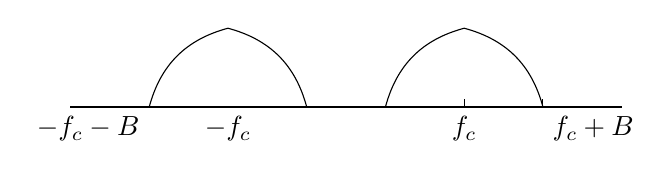
\begin{tikzpicture}
        \draw (0, 0) -- (7, 0);

        \draw (1 , 0) to[bend left] ++(1, 1) to[bend left] ++(1, -1); 
        \node[below] at (2, 0) {$-f_c$};
        \node[below left] at (1, 0) {$-f_c - B$}; 


        \draw (4 , 0) to[bend left] ++(1, 1) to[bend left] ++(1, -1); 
        \draw (5, 0.1) -- ++(0, -0.1) node[below] {$f_c$};
        \draw (6, 0.1) -- ++(0, -0.1) node[below right] {$f_c + B$}; 

    \end{tikzpicture}
    \end{center}

What's the lowest sampling rate we can use to reconstruct this signal?

Certainly, via Nyquist, we need to have $1/T > 2B$. Can we do better? 

Using SSB, we can cut down to $1/T > 2f_c$ (since we only need to sample the sideband).

\section{Feb 24 - Quantization} 

Motivated by the digital domain, we want to represent $m(t)$ as a collection of bits. 

Using Nyquist, we sample 
\[m(t) \to \{m(t_1), m(t_2), \dots, m(t_{N-1})\}\]

\begin{center}
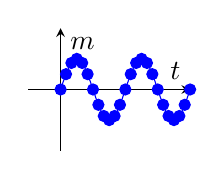
\begin{tikzpicture}
\begin{axis}[
    width=0.3\textwidth,
    axis lines=middle,
    no markers,
    xtick=\empty,
    ytick=\empty,
    clip=false,
    xlabel={$t$},
    ylabel={$m$},
    domain=0:2,
    ymin=-2, ymax=2,
    xmin= -0.5, xmax=2,
    view = {0}{90}
]
    \addplot[blue, samples=100] {sin(2*pi*deg(x))};
    \addplot[blue, samples=25, only marks, mark=o] {sin(2*pi*deg(x))};
\end{axis}
\end{tikzpicture}
\end{center}

We will introduce a \tbf{N-level uniform quantizer} $Q(m)$ which maps $m(t_i)$ to the closest quantization level $q_j$ for $j = 0, \dots, N-1$.

\begin{center}
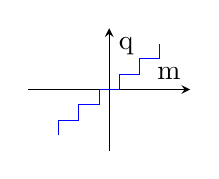
\begin{tikzpicture}
\begin{axis}[
    width=0.3\textwidth,
    axis lines=middle,
    no markers,
    xtick=\empty,
    ytick=\empty,
    clip=false,
    xlabel={m},
    ylabel={q},
    domain=-2:2,
    ymin=-2, ymax=2,
    xmin= -2, xmax=2,
    view = {0}{90}
]
    \addplot coordinates {(-1.25, -1.5) (-1.25, -1) (-0.75, -1) (-0.75, -0.5) (-0.25, -0.5) (-0.25, 0) (0.25, 0) (0.25, 0.5) (0.75, 0.5) (0.75, 1) (1.25, 1) (1.25, 1.5)};
\end{axis}
\end{tikzpicture}
\end{center}

Now, at the receiver we receive a sequence of quantization levels (say $\{q_3, q_1, q_7, q_2, \dots\}$) and we can reconstruct $\hat m(t)$ by using the interpellation formula on the quantized samples.

What if $m(t)$ looks like this?

\begin{center}
\begin{tikzpicture}
    \draw (0, 0) -- (10, 0);
    \draw (5, -2) -- (5, 2); 

    \draw[red, wavy] (2, 1) -- ++(2, 0);
    \draw[red, wavy] (4, -1) -- ++(2, 0);
    \draw[red, wavy] (6, 1) -- ++(2, 0);
    \draw[red] (4, 1) -- (4, -1);
    \draw[red] (6, 1) -- (6, -1);




\end{tikzpicture}
\end{center}

Now all the detail is in the high frequencies so uniform quantization is not good! 

We could try to make the quantization levels smaller but this wastes bits. 

Another option is to tailor the quantizer given knowledge of the signal. Obviously, we can't know the signal exactly at the receiver to design a perfect quantizer but we can use some information about the distribution $f_m$ of $m(t)$ to do better. 

\begin{center}
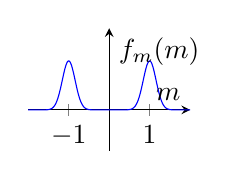
\begin{tikzpicture}
\begin{axis}[
    width=0.3\textwidth,
    axis lines=middle,
    no markers,
    xtick={-1, 1},
    ytick=\empty,
    clip=false,
    xlabel={$m$},
    ylabel={$f_m(m)$},
    domain=-2:2,
    ymin=-0.5, ymax=1,
    xmin= -2, xmax=2,
    view = {0}{90}
]
    \addplot[samples=100, domain=0:2, blue] {0.6*exp(-20*(1-x)^2)};
    \addplot[samples=100, blue, domain=-2:0] {0.6*exp(-20*(1+x)^2)};

\end{axis}
\end{tikzpicture}
\end{center}

If we sample to see the $\P(M < m)$ for various levels $m$, we get the \tbf{cumulative distribution function} (CDF) of $M$, $F_M(m)$, and in fact 
\[f_m(m) = \frac{d}{dm} F_m(m) \]

To review, our scheme looks like 

\begin{center}
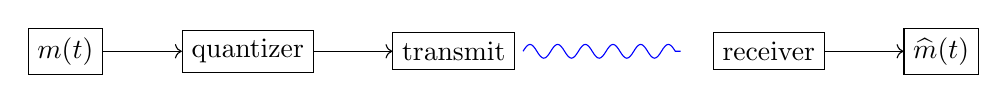
\begin{tikzpicture}
    \node[draw, rectangle] (m) at (0, 0) {$m(t)$};
    \draw[->] (m.east) -- ++(1, 0) node[right, draw, rectangle] (q) {quantizer};
    \draw[->] (q.east) -- ++(1, 0) node[right, draw, rectangle] (t) {transmit};

    \draw[blue, wavy] ($(t.east)+(0.1, 0)$) -- ++(2, 0);
    \node[draw, rectangle] (r) at ($(t)+(4,0)$) {receiver};
    \draw[->] (r.east) -- ++(1, 0) node[right, draw, rectangle] {$\hat m(t)$};


\end{tikzpicture}
\end{center}

though, of course, $m(t) \neq \hat m(t)$ because of loss and quantization error. 

Let $Q(m)$ be the quantization function for some $m$ sampled from $m(t)$. 

Then 
\begin{align*}
    e^2 &= (m - Q(m))^2\\ 
    \bar{e^2} &= \int f_M(m) (m - Q(m))^2 \; dm
\end{align*}
is the \tbf{expected error}

What are the parameters that define a quantizer? Clearly the quantization levels $q_0, \dots, q_{N-1}$ but also the \tbf{decision boundaries} $x_0, \dots$ 


\begin{center}
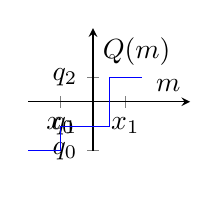
\begin{tikzpicture}
\begin{axis}[
    width=0.3\textwidth,
    axis lines=middle,
    no markers,
    xtick={-1, 1},
    xticklabels={$x_0$, $x_1$},
    ytick={-2, -1, 1},
    yticklabels={$q_0$, $q_1$, $q_2$},
    clip=false,
    xlabel={$m$},
    ylabel={$Q(m)$},
    domain=-2:2,
    ymin=-2, ymax=3,
    xmin= -2, xmax=3,
    view = {0}{90}
]
    \addplot coordinates {(-2, -2) (-1, -2) (-1, -1) (0.5, -1) (0.5, 1) (1.5, 1) };
\end{axis}
\end{tikzpicture}
\end{center}
\[\mathcal Q = \{q_0, q_1, q_2, x_0, x_1\}\]
and we want to find
\[\min_{\mathcal Q} e^2\]

so we take partials, set to zero, solve, and check the second partials for convexity

\begin{exercise}
    \textbf{Exercise:} 
    \[z = x^2 + y^2\]

    \begin{align*}
        \frac{\partial z}{\partial x} &= 2x = 0\\ 
        \frac{\partial z}{\partial y} &= 2y = 0\\ 
        \frac{\partial^2 z}{\partial x^2} &= 2 > 0\\
        \frac{\partial^2 z}{\partial y^2} &= 2 > 0
    \end{align*}

    So convex!

    \div 

    \[z = x^2 + 4xy + y^2\]

    \begin{center}
    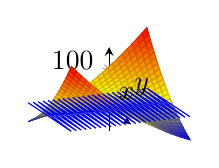
\begin{tikzpicture}
    \begin{axis}[
        width=0.3\textwidth,
        axis lines=middle,
        no markers,
        xtick=\empty,
        ytick=\empty,
        clip=false,
        xlabel={$x$},
        ylabel={$y$},
        view = {70}{20}
    ]
        \addplot3[surf] {x^2 - 4*x*y + y^2};
        \addplot3[blue] {y};
    \end{axis}
    \end{tikzpicture}
    \end{center}

    \begin{align*}
        \frac{\partial z}{\partial x} &= 2x + 4y = 0\\
        \frac{\partial z}{\partial y} &= 2y + 4x = 0\\
        \frac{\partial^2 z}{\partial x^2} &= 2\\
        \frac{\partial^2 z}{\partial y^2} &= 2
    \end{align*}

    But this does not have a global minimum!
\end{exercise}

Let's try this for our error function.
\begin{align*}
    e^2 &= \int (m - Q(m))^2 f_M(m)\; dm\\ 
    &= \int_{-\infty}^{x_0}(m - q_0)^2 f_M(m)\; dm + \int_{x_0}^{x_1} (m - q_1)^2 f_M(m)\; dm + \dots + \int_{x_{N-1}}^{\infty} (m - q_{N-1})^2 f_M(m)\; dm\\ 
    \frac{\partial e^2}{\partial q_i} &= \frac{\partial}{\partial q_i} \int_{x_{i-1}}^{x_i} 2(q_i - m) f_M(m)\; dm\\ 
    &= 2 \int_{x_{i-1}}^{x_i} (m - q_i) f_M(m)\; dm = 0\\ 
    \frac{\partial e^2}{\partial x_i} &= \frac{\partial}{\partial x_i} \left[\int_{x_{i-1}}^{x_i} (m - q_i)^2 f_M(m)\; dm + \int_{x_i}^{x_{i+1}} (m - q_{i+1})^2 f_M(m)\; dm\right]\\
    &= (m - q_i)^2 f_M(x_i) - (m - q_{i+1})^2 f_M(x_i) = 0
\end{align*}
via 
\begin{proposition}
    \textbf{Leibniz's Rule:} 
    \[\frac{d}{dx} \int_{a(x)}^{b(x)} f(x, y)\; dy = f(x, b(x)) \cdot \frac{db}{dx} - f(x, a(x)) \cdot \frac{da}{dx} + \int_{a(x)}^{b(x)} \frac{\partial f}{\partial x}\; dy\]
\end{proposition}
which implies 
\begin{align*}
    (x_i - q_i)^2 &= (x_i - q_{i+1})^2 \\
    x_i^2 - 2 x_i q_i + q_i^2 &= x_i^2 - 2 x_i q_{i+1} + q_{i+1}^2
\end{align*}
\[\boxed{q_i = \frac{q_{i-1} + q_{i+1}}{2}}\]
and 
\[
    \int_{x_{i-1}}^{x_i} m f_M(m)\; dm = q_i \underbrace{\int_{x_{i-1}}^{x_i} f_M(m)\; dm}_{p_m = \P(m \in (x_{i-1}, x_i))}
\]
(assuming $f_M(x_i) \neq 0$) 

At last giving an explicit formula for the quantization levels and decision boundaries:
\[\boxed{q_i = \int_{x_{i-1}}^{x_i} m \frac{f_M(m)}{p_m}\; dm}\]
which is precisely the \emph{conditional average on M} given $M \in (x_{i-1}, x_i)$

Together, these are exactly the \tbf{Lloyd-Max Conditions} for optimal quantization. 

\section{Feb 26 - Lloyd Max Review}

Recall: we sample $m(t) \to \{m_1, m_2, \dots\}$ creating a pdf $f_M(m)$. The intuition is we want to use information from this pdf to design a quantizer that minimizes the expected error while using a reasonable number of quantization levels.

Define an \emph{error function} 
\[e^2 = \int (m - Q(m))^2 f_M(m)\; dm\]
for $Q(m)$ a quantization function defined by quantization levels $q_0, \dots, q_{N-1}$ and breakpoints $x_0, \dots, x_{N-2}$.

Since $Q$ is piecewise constant, we can write
\[e^2 = \int_{-\infty}^{x_0} (m - Q(m))^2 f_M(m)\; dm + \int_{x_0}^{x_1} (m - Q(M))^2 f_M(m)\; dm + \dots + \int_{x_{N-2}}^{\infty} (m - Q(m))^2 f_M(m)\; dm\]

We will blindly take partials using Leibniz and set to zero to minimize. 
\begin{align*}
    \frac{\partial e^2}{\partial x_i} &= \frac{\partial}{\partial x_i} \left[\int_{x_{i-1}}^{x_i} (m - q_{i+1})^2 f_M(m)\; dm + \int_{x_{i-1}}^{x_{i}} (m - q_{i})^2 f_M(m)\; dm\right]\\
    &= -(x_i - q_{i+1})^2 f_M(x_i) + (x_i - q_i)^2 f_M(x_i) = 0
\end{align*}

Assuming $f_M(x_i) \neq 0$, we get
\begin{align*}
    (x_i - q_i)^2 &= (x_i - q_{i+1})^2 \\ 
    x_i^2 - 2 x_i q_i + q_i^2 &= x_i^2 - 2 x_i q_{i+1} + q_{i+1}^2\\
    2(q_{i+1} - q_i) x_i &= q_{i+1}^2 - q_i^2\\
    2(q_{i+1} - q_i) x_i &= (q_{i+1} - q_i)(q_{i+1} + q_i)
\end{align*}
so 
\[\boxed{x_i = \frac{q_{i+1} + q_i}{2}}\]

that is, the breakpoints are the midpoints of the quantization levels - a very nice result!

Now let's go back and take the partials with respect to $q_i$. First let $p_i = \P(m \in (x_{i-1}, x_i))$. 
\begin{align*}
    \frac{\partial e^2}{\partial q_i} &= \frac{\partial}{\partial q_i} \int_{x_{i-1}}^{x_i} 2(q_i - m) f_M(m)\; dm\\ 
    &= 2 \int_{x_{i-1}}^{x_i} (m - q_i) f_M(m)\; dm = 0\\ 
    &= \int_{x_{i-1}}^{x_i} m f_M(m)\; dm - q_i \int_{x_{i-1}}^{x_i} f_M(m)\; dm = 0\\
\end{align*}
so 
\[\int_{x_{i-1}}^{x_i} m f_M(m)\; dm = q_i \int_{x_{i-1}}^{x_i} f_M(m)\; dm\]
hence
\[\boxed{q_i = \int_{x_{i-1}}^{x_i} m \frac{f_M(m)}{p_i}\; dm = \E[M \; | \; m \in (x_{i-1}, x_i)]}\]

Together, the boxed equations are the \tbf{Lloyd-Max Conditions} for optimal quantization. 

If given $\{x_i\}$, the optimal $\{q_i\}$ are given by the conditions. Similarly, if given $\{q_i\}$, the optimal $\{x_i\}$ are given by the conditions. 

In particular, this optimality ensures the quantizer will be monotonic since it intuitively should correspond to ``binning'' the amplitudes of the samples. 

\begin{exercise}
    \textbf{Exercise:} Prove that the Lloyd-Max conditions are optimal (Hint: see quantization notes on canvas)
\end{exercise}

As we will see, our error function is \emph{convex}. 

\tbf{Convexity (according to high school calculus):} $f(x)$ convex iff $\frac{d^2f(x)}{dx^2} > 0 \quad \forall x$ 

\tbf{Convexity (for adults):} $f(x_1, \dots, x_n)$ convex iff $\forall x_1, x_2 \in \R^n$ and $\lambda \in [0, 1]$, 
\[f(\lambda x_1 + (1 - \lambda)x_2) \leq \lambda f(x_1) + (1 - \lambda) f(x_2) \] 
(corresponding to a chord between any two points of $f$ being above the curve)

\tbf{Strictly convex:} $f$ is strictly convex if the above inequality is strict for $\lambda \in (0, 1)$

\begin{exercise}
    \textbf{Exercise:} Show that the two convexity definitions are equivalent. (Hint: use the Hessian)
\end{exercise}

\chapter{Interlude - Introduction to Probability and Stochastic Processes}
\section{March 3}
    \tbf{Random variable:} a map $X: \Omega \to \R$ for $\Omega$ an \emph{event space}. 

    This map can take single events or sets of events as input. (Imagine for example the probability of rolling a 2 on two dice (one possibility) vs the probability of rolling a 7 on at least one die (multiple possibilities))

    \tbf{Probability Mass Function (pmf):} $\{\omega_1, \dots, \omega_n\} \to \{p_1, \dots, p_n\}$ where $p_i = \P(\omega_i)$ satisfying 
    \begin{enumerate}
        \item $\sum_{i=1}^n p_i = 1$. 
        \item $p_i \geq 0$ for all $i$.
    \end{enumerate} 

    \tbf{Cumulative distribution function (cdf):} $P(x) = \P(X \leq x)$ for a random variable $X$. 
 
    \tbf{Expectation:} $\E[X] = \sum_{i=1}^n p_i X(\omega_i) := \bar X$

    \emph{Examples:} 
    \begin{itemize}
        \item $\E[X^2] = \sum_{i=1}^n p_i X(\omega_i)^2$
        \item $\E[f(X)] = \sum_{i=1}^n p_i f(X(\omega_i))$ 
    \end{itemize}

    \tbf{Property:} Expectation is linear: 
    \[\E[f(X) + g(Y)] = \sum p_n (f(X) + g(Y)) = \sum p_n f(X) + \sum p_n g(Y) = \E[f(X)] + \E[g(Y)]\]

    \begin{exercise}
        \textbf{Exercise:} Calculate $\E[(X - \bar X)^2]$ 

        \div 
        \begin{align*}
            \E[(X - \bar X)^2] &= \sum_{i=1}^n p_i (X(\omega_i) - \bar X)^2\\ 
            &= \sum_{i=1}^n p_i (X(\omega_i)^2 - 2 X(\omega_i) \bar X + \bar X^2)\\
            &= \sum_i p_i X_i^2 - 2 \bar X \sum p_i X_i + \bar X \sum p_i\\ 
            &=  \E[X^2] - 2 \bar X \cdot \bar X + \bar X^2\\
            &= \E[X^2] - \bar X^2\\ 
            &= \Var[X]
        \end{align*}
    \end{exercise}

    \tbf{Examples of PMFs:}
    \begin{enumerate}
        \item Uniform 
        
        \begin{center}
        \begin{tikzpicture}
            \draw (0, 0) -- (6, 0); 
            \draw (0, -0.5)  -- ++(0, 1); 

            \foreach \x in {1, ..., 5} {
                \draw[blue] (\x, 0) -- (\x, 0.5) node {$\circ$}; 
            }
        \end{tikzpicture}
        \end{center}

        \item Poisson 
        \[p_{\lambda}(k) = \frac{(\lambda T)^k}{k!} e^{-\lambda T}, \quad k = 0, 1, 2, \dots\] 
        (nicely satisfying $\E[K] = \lambda T$)

        \item Geometric 
        \[p_{\alpha}(k) = (1 - \alpha) \alpha^k, \quad \alpha \in [0, 1], \; k = 0, 1, 2, \dots\]
        (recall $\sum_{k=0}^{\infty} \alpha^k = 1/(1 - \alpha)$) 

        \begin{center}
        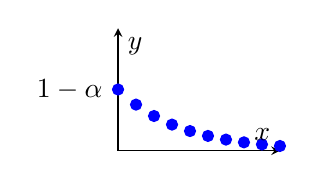
\begin{tikzpicture}
        \begin{axis}[
            width=0.3\textwidth,
            axis lines=middle,
            no markers,
            xtick=\empty,
            ytick={1},
            yticklabels={$1 - \alpha$},
            clip=false,
            xlabel={$x$},
            ylabel={$y$},
            ymin=0, ymax=2,
            xmin=0, xmax=5,
            view = {0}{90}
        ]
            \addplot[blue, domain=0:5, samples=10, only marks, mark=o]  {0.6^x}; 
        \end{axis}
        \end{tikzpicture}
        \end{center}

        \item Binomial 
        \[p_{\alpha}(k) = \binom{N}{k} \alpha^k (1 - \alpha)^{N-k}\] 
        for $k$ the number of heads in $N$ Bernoulli trial with $\P(H) = \alpha$ and $\P(T) = 1 -\alpha$ 

        (notice $\E[K] = \alpha K$)

    \end{enumerate}

    Now let's move on to \tbf{continuous random variables} where we have a \tbf{probability density function (pdf)} $f_X(x)$ such that
    \begin{enumerate}
        \item $f_X(x) \geq 0$ for all $x$.
        \item $\int_{-\infty}^{\infty} f_X(x)\; dx = 1$
    \end{enumerate} 
    and a \tbf{cumulative distribution function (CDF)}
    \[F_X(x) = \int_{-\infty}^x f_X(\xi)\; d\xi = \P(X \leq x)\]

    \tbf{Expection of a continuous RV:} 
    \[\E[X] = \int x f_X(x)\; dx := \bar X\]

    \tbf{Variance of a continuous RV:} 
    \[\Var[X] = \E[(X - \bar X)^2] = \int (x - \bar X)^2 f_X(x)\; dx = \E[X^2] - \E[\bar X]^2 = \E[X^2] - \bar X^2 = \sigma_X^2\]

    Notice that from the definition of the CDF, we have 
    \[F_X(x) = \int_{-\infty}^x f_X(y)\; dy \iff f_X(x) = \frac{d}{dx} F_X(x)\]
    
    \tbf{Joint Random Variables:} Let $X, Y$ be two random variables with joint pdf $f_{X, Y}(x, y)$ satisfying
    \begin{enumerate}
        \item $\int \int f_{X, Y}(x, y)\; dx\, dy = 1$
        \item $f_{X, Y}(x, y) \geq 0$ for all $x, y$.
    \end{enumerate}

    notice that this first property leads to the \tbf{marginal pdfs}
    \begin{align*}
        f_X(x) &= \int f_{X, Y}(x, y)\; dy\\ 
        f_Y(y) &= \int f_{X, Y}(x, y)\; dx
    \end{align*}
    hence 
    \begin{align*}
        \E[X] &= \bar X = \int \int x f_{X, Y}(x, y)\; dx\, dy\\
        \E[Y] &= \bar Y
    \end{align*}

    Notice that we do not know that $X$ and $Y$ are independent. 

    Consider these two examples:
    \begin{center}
        \begin{multicols}{2}
            \begin{center}
            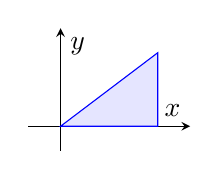
\begin{tikzpicture}
            \begin{axis}[
                width=0.3\textwidth,
                axis lines=middle,
                no markers,
                xtick=\empty,
                ytick=\empty,
                clip=false,
                xlabel={$x$},
                ylabel={$y$},
                domain=0:1.5,
                ymin=-0.5, ymax=2,
                xmin= -0.5, xmax=2,
                view = {0}{90}
            ]
                \addplot[blue, fill, fill opacity=0.1] {x} \closedcycle;
            \end{axis}
            \end{tikzpicture}
            \end{center}

            \begin{center}
            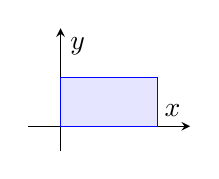
\begin{tikzpicture}
            \begin{axis}[
                width=0.3\textwidth,
                axis lines=middle,
                no markers,
                xtick=\empty,
                ytick=\empty,
                clip=false,
                xlabel={$x$},
                ylabel={$y$},
                domain=0:1.5,
                ymin=-0.5, ymax=2,
                xmin= -0.5, xmax=2,
                view = {0}{90}
            ]
                \addplot[blue, fill, fill opacity=0.1] {1} \closedcycle;
            \end{axis}
            \end{tikzpicture}
            \end{center}
        \end{multicols}
    \end{center}

    If we know $X \cdot Y = 1$, then in the first example, knowing $X = 0$ fixes $Y$. In the second case, knowing $X = 0$ only tells us that $Y \sim \text{Unif}(0, 1)$ -- no new information. 

    \tbf{Conditional probability:}
    \[f_{X |Y}(x\; | \; y) = \frac{f_{X, Y}(x, y)}{f_Y(y)}\]
    (the joint pdf divided by the marginal pdf of $Y$)

    \tbf{Bayes' Theorem:} 
    \[f_{X, Y}(x, y) = f_{X |Y}(x\; | \; y) f_Y(y) = f_{Y  | X}(y \; | \; x) f_X(x)\]

    \tbf{Independence:} $X$ and $Y$ are independent iff 
    \[f_{X | Y} (x \; | \; y) = f_X(x)\] 
    Intuitively,, telling me $y$ tells me nothing about $x$.  

    \begin{exercise}
        \textbf{Exercise:} Show that for independent $X, Y$ 
        \[f_{X, Y}(x, y) = f_X(x) f_Y(y)\]
    \end{exercise}
    
    \tbf{Correlation:} 
    \[\E[XY] = \int \int x\, y\; f_{X, Y} (x, y) \; dx\, dy\]
    which is precisely $\E[X] \cdot \E[Y]$ for independent $X, Y$

    \tbf{Covariance:}
    \[\E[(X - \bar X)(Y - \bar Y)] = \int \int (X - \bar X)(Y - \bar Y) f_{X, Y}(x, y)\; dx\, dy\]
    and since $\E[X - \bar X] = 0$, we have that the covariance is \emph{zero} for independent $X, Y$

    \tbf{Gaussian:}
    \[f_X(x) = \frac{1}{\sqrt{2\pi \sigma^2}} e^{-\frac{(x - \mu)^2}{2\sigma^2}}\]

    \begin{center}
    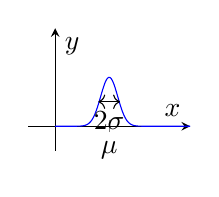
\begin{tikzpicture}
    \begin{axis}[
        width=0.3\textwidth,
        axis lines=middle,
        no markers,
        xtick={2},
        xticklabels={$\mu$},
        ytick=\empty,
        clip=false,
        xlabel={$x$},
        ylabel={$y$},
        domain=0:5,
        ymin=-0.5, ymax=2,
        xmin= -1, xmax=5,
        view = {0}{90}
    ]
        \addplot[blue, samples=100] {exp(-5*(x-2)^2)};
        \draw [<->] (1.6, 0.5) -- (2.4, 0.5) node[midway, below] {$2\sigma$};
    \end{axis}
    \end{tikzpicture}
    \end{center}

    \tbf{Joint Gaussian:}
    \[f_X(x_1, \dots, x_N) = \left(\frac{1}{2\pi}\right)^{N/2} \abs{K}^{-1/2} \exp\left(\frac{-(\vec x - \vec \mu)^{\top} K^{-1} (\vec x - \vec \mu)}{2}\right) \]
    for covariance matrix 
    \[K = \E[( \vec{x} - \vec \mu)(\vec x - \vec \mu)^{\top}] = \begin{pmatrix}
        \sigma_1^2 & \Cov[X_1, X_2] & \dots & \Cov[X_1, X_N]\\
        \Cov[X_2, X_1] & \sigma_2^2 & \dots & \Cov[X_2, X_N]\\
        \vdots & \vdots & \ddots & \vdots\\
        \Cov[X_N, X_1] & \Cov[X_N, X_2] & \dots & \sigma_N^2
    \end{pmatrix}\]
    
    \begin{proposition}
        \textbf{Theorem:} If $X, Y$ are jointly Gaussian, 
        \[\Cov(X, Y) = 0 \implies X \perp Y\]
        and for any $X, Y$ independent 
        \[X \perp Y \implies \Cov(X, Y) = 0\]
    \end{proposition}

    \tbf{Adding Random Variables:} Suppose $Z = X + Y$. Given $f_{X, Y}(x, y)$, what is $F_Z(z)$?

    First, 
    \[\P(Z \leq z) = \P(X + Y \leq z)\]

    \begin{center}
    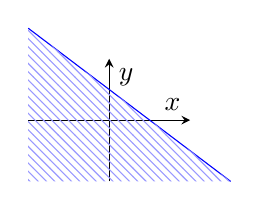
\begin{tikzpicture}
    \begin{axis}[
        width=0.3\textwidth,
        axis lines=middle,
        no markers,
        xtick=\empty,
        ytick=\empty,
        clip=false,
        xlabel={$x$},
        ylabel={$y$},
        domain=-2:3,
        ymin=-2, ymax=2,
        xmin= -2, xmax=2,
        view = {0}{90}
    ]
        \addplot[fill, fill opacity=0.1, blue] {1 - x};
        \draw[draw=none,pattern=north west lines, pattern color=blue!40] (-2, 3)--(3, -2)--(-2,-2)--cycle;
    \end{axis}
    \end{tikzpicture}
    \end{center}

    Hence 
    \begin{align*}
        \P(Z \leq z) &= \int_{-\infty}^{\infty} \int_{-\infty}^{z-x} f_{X, Y}(x, y) \; dy\, dx\\ 
        &= \int_{-\infty}^{\infty} \int_{-\infty}^{z-x} f_{X}(x) f_Y(y) \; dy\, dx \qquad (X \perp Y)\\
        \frac{d}{dz} \P(Z \leq z) &= \int_{-\infty}^{\infty} f_X(x) \cdot f_Y(z-x) \; dx \qquad \text{(Leibniz)}\\ 
        &= (f_X \star f_Y)(z)
    \end{align*}

    Convolution!!
    
    Example, if $Z = X + Y$ for $X, Y \iid \text{Unif}(-1, 1)$, then
    \begin{center}
    \begin{tikzpicture}
    \begin{axis}[
        width=0.3\textwidth,
        axis lines=middle,
        axis equal,
        no markers,
        xtick=\empty,
        ytick=\empty,
        clip=false,
        xlabel={$z$},
        ylabel={$f_Z(z)$},
        domain=-2:2,
        ymin=-0.5, ymax=2,
        xmin= -2, xmax=2,
        view = {0}{90}
    ]
        \addplot[blue, domain=-1:0] {1+x};
        \addplot[blue, domain=0:1] {1-x};

    \end{axis}
    \end{tikzpicture}
    \end{center}

    We have seen this over an over. Now what happens if we take $Z + Z$? 
    
    \begin{center}
        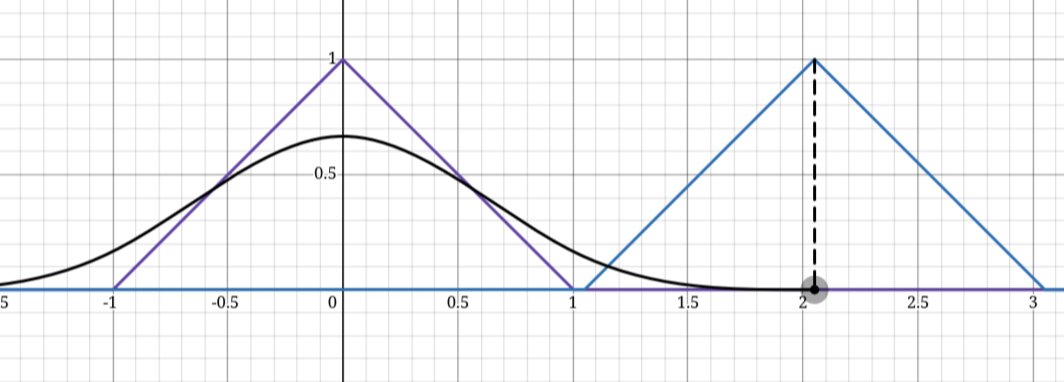
\includegraphics[width=0.5\textwidth]{Images/iterated_convolution.png}
    \end{center}

    We find that it smooths out. What happens if we keep iterating?

    \tbf{Central limit theorem:} For $X_k$ iid, 
    \[\lim_{n \to \infty} \frac{1}{\sqrt n} \sum_{k=1}^n (X_k - \bar X)  \to \Nc(0, \sigma^2)\]

\section{March 5 - Gaussians and Stochastic Processes}

\subsection{Gaussians} 

\tbf{Univariate Gaussian:}
\[f_{\mu, \sigma}(x) = \frac{1}{\sqrt{2\pi\sigma^2}} \exp\left(-\frac{1}{2} \left(\frac{x - \mu}{\sigma}\right)^2\right)\]

\tbf{Multivariate Gaussian:}
\[f_{K, \vec mu} = \left(\frac{1}{2\pi}\right)^{N/2} \abs{K}^{-1/2} \exp\left(-\frac{1}{2} (\vec x - \vec \mu)^{\top} K^{-1} (\vec x - \vec \mu)\right)\] 

Consider the case where $\vec X = (X_1, X_2)^{\top}$. What do we need to know to find the joint Gaussian pdf? Only the mean $\vec \mu$ and the covariance matrix $K$.
\[K = \E\begin{bmatrix}
    \Var X_1 & \Cov[X_1, X_2]\\
    \Cov[X_2, X_1] & \Var X_2
\end{bmatrix} = \E\begin{bmatrix}
    (X_1 - \mu_1)^2 & (X_1 - \mu_1)(X_2 - \mu_2)\\
    (X_2 - \mu_2)(X_1 - \mu_1) & (X_2 - \mu_2)^2
\end{bmatrix} = \E[(\vec X - \vec \mu)^{\top}(\vec x - \vec \mu)]\]

\emph{Notation:} $\Var X_1 = \sigma_1^2$ and $\Cov[X_1, X_2] = \rho_{12}$

What if $\rho_{12} = \rho_{21} = 0$? Then 
\[K = \begin{pmatrix}
    \sigma_1^2 & 0\\ 
    0 & \sigma_2^2
\end{pmatrix}\]
so 
\[K^{-1} = \begin{pmatrix}
    1/\sigma_1^2 & 0\\ 
    0 & 1/\sigma_2^2
\end{pmatrix}, \qquad \abs K = \sigma_1^2 \sigma_2^2\]
hence 
\begin{align*}
    f_{K, \vec \mu}(x) &= \left(\frac{1}{2\pi}\right) \frac{1}{\sqrt{\sigma_1^2 \sigma_2^2}} \,\exp\left(-\frac{1}{2} \begin{pmatrix}
        x_1 - \mu_1\\ 
        x_2 - \mu_2
    \end{pmatrix}^{\top} \begin{pmatrix}
        1/\sigma_1^2 & 0\\ 
        0 & 1/\sigma_2^2
    \end{pmatrix} \begin{pmatrix}
        x_1 - \mu_1\\ 
        x_2 - \mu_2
    \end{pmatrix}\right)\\ 
    &= \left(\frac{1}{2\pi}\right) \frac{1}{\sqrt{\sigma_1^2 \sigma_2^2}} \,\exp\left(-\frac{1}{2} \left[\frac{(x_1 - \mu_1)^2}{\sigma_1^2} + \frac{(x_2 - \mu_2)^2}{\sigma_2^2}\right]\right)\\
    &= \frac{1}{\sqrt{2\pi \sigma_1^2}} e^{-(x_1 - \mu_1)^2/(2\sigma_1^2)} \cdot \frac{1}{\sqrt{2\pi \sigma_2^2}} e^{-(x_2 - \mu_2)^2/(2\sigma_2^2)}\\
    &= f_{\mu_1, \sigma_1}(x_1) \cdot f_{\mu_2, \sigma_2}(x_2)
\end{align*}

\begin{proposition}
    \textbf{Proposition:} If $\vec X$ is a set of jointly Gaussian RVs and all their covariances are zero, they are independent. 
\end{proposition}

As we will see, joint Gaussian RVs have some very nice properties. 

Let $X_1 \sim \Nc(\mu_1, \sigma_1^2)$ and $X_2 \sim \Nc(\mu_2, \sigma_2^2)$ be independent (\emph{Notation:} $X_1 \perp X_2$). What is the distribution of $Z = X_1 + X_2$? 

\begin{tbox}{\textbf{Lemma:} For $X, Y$ independent and $Z = X + Y$, $\Var Z = \Var X + \Var Y$
}
    \emph{Proof:} 
    \begin{align*}
        \E[Z^2] &= \E[(X - \bar X + Y - \bar Y)^2 ]\\ 
        &= \E[(X - \bar X)^2] + \E[(Y - \bar Y)^2] + 2\E[(X - \bar X)(Y - \bar Y)]\\
        &= \Var X + \Var Y + 2 \underbrace{\Cov(X, Y)}_{= 0}\\
        &= \sigma_1^2 + \sigma_2^2 
    \end{align*}
\end{tbox}

\begin{exercise}
    \textbf{Exercise:} Prove that $Z = X + Y \sim \Nc(\mu_1 + \mu_2, \sigma_1^2 + \sigma_2^2)$
\end{exercise}

\begin{proposition}
    \textbf{Proposition:} Let $\vec X, \vec Y$ be jointly Gaussian. Then for $A, B$ linear operators, 
    \begin{enumerate}
        \item $Z = A\vec X$ is jointly Gaussian 
        \item $Z = A \vec X + B \vec Y$ is jointly Gaussian 
    \end{enumerate}
\end{proposition}

Let $X \sim \Unif([0, 1]) = u(x) - u(x - 1)$, for $u$ the unit step. 

\begin{center}
\begin{tikzpicture}
\begin{axis}[
    width=0.3\textwidth,
    axis lines=middle,
    no markers,
    xtick={1},
    ytick={1},
    clip=false,
    xlabel={$x$},
    ylabel={$y$},
    domain=-2:2,
    ymin=-0.5, ymax=2,
    xmin= -0.5, xmax=2,
    view = {0}{90}
]
    \addplot[blue] coordinates {(0, 1) (1, 1) (1, 0)};
\end{axis}
\end{tikzpicture}
\end{center}

Now let $Y = X^2$. What is the CDF of $Y$? 

\[F_Y(y) = \P(Y \leq y) = \P(X^2 \leq y) = \P(X \leq \sqrt y) = \sqrt y\]
hence 
\[f_Y(y) = \frac{d}{dy} F_Y(y) = \frac{1}{2\sqrt y}\]

\subsection{Stochastic Processes}

\tbf{Recall:} A random variable $X$ is a mapping from event space $X: \Omega \to \R$. 

\tbf{Random process:} A random process is a mapping from event space to functions $X: \omega \mapsto f(t, \omega)$. 

If we know $t$, this is just a random variable. If we know $\omega$, this is a random function. If we know both, this is just a number.

Say we have a graph of Chris' position over time and we want to predict where he will be at time $t$ to throw a dart at him. We can model his position as a random process $X(t)$. 

What are some things we might want to know about this process?
\begin{itemize}
    \item $\bar X(t) = \E[X(t)]$ - the expected position at time $t$
    \item $\Var[X(t)] = \E[X(t) - \bar X(t)]$ - the variance of his position at time $t$
    \item $\rho_X(t, \tau) = \E[X(t) X(t + \tau)]$ - the correlation of his position at time $t$ and $t + \tau$ (how much does knowing his position at time $t$ tell us about his position at time $t + \tau$?)
\end{itemize}

\tbf{Remark:} in this class, we will assume all processes are \emph{stationary:} $\rho_X(t, \tau) = \rho(\tau)$ for all $t$.

What we would really like, though, is to know the \tbf{joint distribution} of $X(t_1), \dots, X(t_n)$ for all $n$ and $t_1, \dots, t_n$ with $n$ very large. In theory, this gives us full knowledge of the process. In practice, this is impossible to know, so we will make some assumptions about the process to make it tractable.

\tbf{Stationary Gaussian Process:} $\{X_t: t \in \Z\}$ is a stationary Gaussian process if 
\begin{enumerate}
    \item $\E[X(t)] = 0$
    \item $\E\bigg[\big(X(t) - \E[X(t)]\big)\big(X(t + \tau) - \E[X(t + \tau)]\big)\bigg] = K(\tau)$
\end{enumerate}

In particular, this means that if we know the mean and covariance function of a stationary Gaussian process, we know the full joint distribution of the process -- precisely what we said was impossible to know in general.

\tbf{White Gaussian Process:} A stationary Gaussian process with 
\[K_X(\tau) = N_0 \delta(\tau) \E[X(t) X(t + \tau)]\] 
for $N_0 \in \R$.

Why is it called white? Consider its \tbf{spectral density}
\[S_X(f) = \F[K_X(\tau)] = \F[N_0 \delta(\tau)] = N_0\] 
which is constant across all frequencies, hence the name white (like white light which contains all frequencies of visible light).

\section{March 10}

\tbf{Recall:} a jointly Gaussian distribution is given by
\[\left(\frac{1}{2\pi}\right)^{N/2} \abs{K}^{-1/2} \exp\left(-\frac{1}{2} (\vec x - \vec \mu)^{\top} K^{-1} (\vec x - \vec \mu)\right) \]
which requires only the mean and the covariance matrix to specify completely (first and second moments).

\begin{align*}
    R_X(\tau) &= \E[X(t) X(t + \tau)]\\
    K_X(\tau) &= \E[(X(t) - \mu)(X(t + \tau) - \mu)]\\ 
    R_{XY}(\tau) &= \E[X(t) Y(t + \tau)]
\end{align*}

Last time, we started talking about stochastic processes because signals are random due to noise, interference, and other factors. Today, we will start thinking about \emph{communications in the face of noise.}

For a random process, we need to know the joint distribution $f_{X(t_1), \dots, X(t_n)}(x_1, \dots, x_n)$ for all $n$ and $t_1, \dots, t_n$ to completely characterize it (even ignoring the fact that there are uncountably many $t$). This is HARD. But Gaussians are wonderful! 

For a stationary Gaussian process, given $m$ (constant because stationary) and $K(\tau)$, what is $f_{X(t_1), X(t_2)}(x_1, x_2)$?

In particular, what is the relationship between the covariance function $K(\tau)$ and the covariance matrix $K$? 

\[K = \E\left[\begin{pmatrix}
    X(t_1)\\ X(t_2)
\end{pmatrix}\begin{pmatrix}
    X(t_1) & X(t_2)
\end{pmatrix}\right] = \begin{pmatrix}
    K(0) & K(t_1 - t_2)\\
    K(t_2 - t_1) & K(0)
\end{pmatrix}\]
(though we have real symmetry, so $K(t_1 - t_2) = K(t_2 - t_1)$)

Then, letting $m = 0$ for simplicity, we have
\[f_{X(t_1), X(t_2)}(x_1, x_2) = \frac{1}{2\pi} \abs{K}^{-1/2} \exp\left(-\frac{1}{2} \vec x^{\top} K^{-1} \vec x\right)\]

Suppose we input a gaussian process into a linear time-invariant (LTI) system with impulse response $h(t)$. What is the output?
\[Y(t) = X(t) \star h(t) = \int_{-\infty}^{\infty} X(\tau) h(t - \tau) d\tau \]
for each $t, \tau$ this is just a linear combination of Gaussian RVs, hence $Y(t)$ is also a Gaussian process. 

What is the mean of $Y(t)$? Let's assume $\E[X(t)] = 0$ and stationary for simplicity. Then
\[\E[Y(t)] = \int \int X(\tau) h(t - \tau) \; d\tau \, dt = \int h(t - \tau) \E[X(t)] \; d\tau = 0\]

What about the covariance? Changing the variables of integration, 
\begin{align*}
    \E[Y(t) Y(t + \tau)] &= \E\left[\left(\int X(\lambda) h(t - \lambda)\; d\lambda\right)\left(\int X(\sigma) h(t + \tau - \sigma)\; d\sigma\right)\right]\\ 
    &= \E\left[\int \int X(\lambda) X(\sigma) h(t - \lambda) h(t + \tau - \sigma)\; d\sigma d\lambda\right]\\ 
    &= \E\left[\int \int K_X(\lambda - \sigma) h(t - \lambda) h(t + \tau - \sigma)\; d\lambda\, d\sigma\right]
\end{align*}
since
\[K_X(\tau) = \textcolor{red}{\E[X(t_1) X(t_2)]} = \E[X(t_1) X(t_1 + \underbrace{(t_2 - t_1)}_{\tau})] = K_X(t_2 - t_1)\] 

Now, if we further assume this is a white Gaussian process ($K_X(\lambda - \sigma) = N_0 \delta(\lambda - \sigma)$), then
\begin{align*}
    \E[Y(t) Y(t + \tau)] &= \dots\\ 
    &= \E\left[\int \int K_X(\lambda - \sigma) h(t - \lambda) h(t + \tau - \sigma)\; d\lambda\, d\sigma\right]\\ 
    &= N_0 \int h(t - \sigma) h(t + \tau - \sigma) \; d\sigma\\ 
    &= K_Y(\tau)
\end{align*}

Is this actually a function of $t$? Yes. Consider $z = t - \sigma$ then for all $t$, 
\[K_Y(\tau) = N_0 \int h(z) h(z + \tau)\; d\tau \implies \text{ still stationary (only the offset changes)}\]

\subsection{Signalling} 

Define a signalling interval $(0, T)$. We will send a single bit of information $b \in \{-1, 1\}$. 

Sent through the channel, we receive $y(t)$ and want to do some magic to recover $\hat b$ as accurately as possible.

We can model the channel as adding a stationary, white, zero-mean noise $w(t)$ (that is, $\E[w(t)w(t + \tau)] = N_0 \delta(\tau)$) to the signal, so
\[y(t) = x(t) + w(t)\]

Our ability to decode the message then clearly depends on how large the noise $w$ is. 

Let's put $y(t)$ into an LTI with impulse response $h(t)$, outputting $z(t)$. We will sample $z(T)$ to decide if $\hat b = -1$ or $\hat b = 1$. 

\[y(t) = bx(t) + w(t) \implies z(t) = \underbrace{b \int x(\tau) h(t - \tau)\; d\tau}_{\text{info}} + \int w(\tau) h(t + \tau)\; d\tau\]
so 
\[z(T) = \int_0^T x(\tau) h(T - \tau)\; d\tau + \int_0^T w(\tau)h(T - \tau) \; d\tau\]

We know that both are zero in expectation so how can we measure the relative sizes of each? 

\tbf{Signal to noise ratio (SNR):} 
\begin{align*}
    \text{SNR} &= \frac{\E\left[\left(b \int_0^T x(\tau) h(T - \tau)\; d\tau\right)^2\right] }{\E\left[\left(\int_0^T w(\tau) h(T - \tau)\; d\tau\right)^2\right] }\\ 
    &= \frac{\left(\int_0^T x(\tau) h(T - \tau)\; d\tau\right)^2 \E[b^2]}{\E\left[\int \int w(\tau) w(\lambda) h(T - \tau) w(T - \lambda) \; d\tau\, d\lambda\right]}\\ 
    &= \frac{\left(\int_0^T x(\tau) h(T - \tau)\; d\tau\right)^2}{\int_0^T \int_0^T N_0 \delta(\tau - \lambda) h(T - \tau) h(T - \lambda)\; d\tau\, d\lambda}\\ 
    &= \frac{\left(\int_0^T x(\tau) h(T - \tau)\; d\tau\right)^2}{N_0 \int_0^T h^2(T - \lambda)\; d\lambda}\\ 
\end{align*}
where $\Ec_h = N_0 \int_0^T h^2(T - \lambda)\; d\lambda$ is the \tbf{energy} of $h$ (integral of a square!) 

In particular, this means we want to find an $h$ to maximize this ratio. 

We know 
\[\left(\int_0^T x(\tau) h(T - \tau)\; d\tau\right)^2 \leq \left(\int_0^T x^2(\tau)\; d\tau\right)\left(\int_0^T h^2(T - \tau)\; d\tau\right)\]
by Cauchy-Schwarz. 

\begin{proposition}
    \textbf{Cauchy-Schwarz:} 
    \[\left(\int x(t) y(t)\right)^2 \leq \left(\int \abs{x(t)}^2\; dt\right)\left(\int \abs{y(t)}^2\; dt\right)\]
    with equality iff $x(t) \propto y(t)$.  
\end{proposition}

And since we want to maximize the numerator, we want equality. That is, the optimal $h$ is precisely $h(t - \tau) = \alpha x(\tau)$ for $\alpha \in \R$. In which case, 

\[\max\, \text{SNR} = \frac{\left(\int_0^T x^2(\tau)\; d\tau\right) \alpha^2 \int_0^T x^2(\tau)\; d\tau}{N_0 \alpha^2 \int x^2(\tau)\; d\tau} = \frac{\int_0^T x^2(\tau)\; d\tau}{N_0} = \frac{\Ec_x}{N_0}\]

Hence, which LTI system maximizes SNR? Precisely the \emph{matched filter} which scales a flipped version of $x$, resulting in an SNR equal to the quotient of the energy in $x$ and the inherent noise level. 

This means that we don't need to spend much time designing a careful $x$: we just want to maximize energy! 

Recall 
\[z(T) = \int_0^T x(\tau) h(T - \tau)\; d\tau + \int_0^T w(\tau)h(T - \tau) \; d\tau\]
now with the matched filter $h(T - \tau) = x(\tau)$, 
\[Z(T) = b \Ec_x + W\]
with $W = \int_0^T w(\tau) h(T - \tau)\; d\tau \sim \Nc(0, N_0 \Ec_x)$
\[\E[W^2] = \E[\int_0^T \int_0^T w(\tau) w(\lambda) x(\tau) x(\lambda)\; d\tau \, d\lambda] = N_0 \Ec_x\]

If $b = 1$, what does $Z(T)$ look like? 

\begin{center}
\begin{tikzpicture}
\begin{axis}[
    width=0.3\textwidth,
    axis lines=middle,
    no markers,
    xtick={-2, 2},
    xticklabels={$-b\Ec_x$, $b\Ec_x$},
    ytick=\empty,
    clip=false,
    xlabel={$x$},
    ylabel={$y$},
    ymin=0, ymax=2,
    xmin= -5, xmax=5,
    view = {0}{90}
]
    \addplot[blue, samples=100] {exp(-5*(x-2)^2)} node[above] at (axis cs:2,1) {$f_{X\; | \; b = 1}$};
    \addplot[blue, samples=100] {exp(-5*(x+2)^2)} node[above] at (axis cs:-2,1) {$f_{X \; | \; b = -1}$};
\end{axis}
\end{tikzpicture}
\end{center}

as we will see, if we sample at $Z(T)$, we will then be very likely to correctly decode $b$ as $1$ or $-1$ depending on the marginals. 

What if the distributions are more closely overlapping or not so simple? This will be our focus moving forward.

\section{March 12}

\tbf{Quick review:} For a Gaussian random process $w(t)$, a particular sample $w(t_i) \sim \Nc(\mu(t), K(t, \tau))$. If we know the process is stationary, then $w(t_i) \sim \Nc(\mu, K(\tau))$ (only depends on the offset $\tau$).

What do we know about two samples $w(t_1), w(t_2)$? They are jointly Gaussian. And indeed, any finite collection of samples $w(t_1), \dots, w(t_n)$ are jointly Gaussian.

Last time, we combined the entire course thus far to derive the optimal filter for decoding a bit sent through a noisy channel: 

\begin{center}
\begin{tikzpicture}
    \node (m) at (0, 0) {$m(t)$}; 
    \node[draw, rectangle] (s) at (3, 0) {Sampler};
    \node (mk) at (7, 0) {$\{m_1, m_2, \dots, m_k\}$}; 
    \node[draw, rectangle] (q) at (10, 0) {Q};
    \node (b) at (13, 0) {bits $b_1, \dots, b_k$};

    \draw[->] (m) -- (s.west);
    \draw[->] (s.east) -- (mk);
    \draw[->] (mk) -- (q.west);
    \draw[->] (q.east) -- (b);
\end{tikzpicture}
\end{center}
where the sampler is lossless but the quantizer is not (pigeonhole principle).

Now we want to transmit a but $b \in \{-1, 1\}$. We multiply by a carrier $x(t)$ and transmit through a noisy channel to receive $r(t) = b x(t) + w(t)$ where $w(t)$ is a stationary, white Gaussian process with power spectral density $N_0$.

\begin{center}
\begin{tikzpicture}
    \node (y) at (0, 0) {$bx(t) + w(t)$}; 
    \node (r) at (3, 0) {$r(t)$}; 
    \node[draw, rectangle] (h) at (5, 0) {magic}; 
    \node (b) at (7, 0) {$\hat b$};

    \draw[->] (y) -- (r);
    \draw[->] (r) -- (h.west);
    \draw[->] (h.east) -- (b);
\end{tikzpicture}
\end{center}
Our job is to find a system that will decode $r(t)$ to recover $\hat b$. 

Last time, we started with the assumption that the ``magic system'' is an LTI with impulse response $h(t)$. Motivated by trying to maximize the signal to noise ratio, we found that the optimal $h$ is precisely the matched filter $h(t) = x(T - t)$ which results in an SNR of $\Ec_x/N_0$ where $\Ec_x$ is the energy of $x$.

\begin{center}
\begin{tikzpicture}
    \node (y) at (0, 0) {$bx(t) + w(t)$}; 
    \node[draw, rectangle] (h) at (5, 0) {$h(t) = x(T - t)$}; 
    \node[below] at (h.east) at (7, 0) {$y(t)$};
    \node (T) at (9, 0) {$y(T)$};
    
    \draw[->] (y) -- (h.west); 
    \draw (h.east) -- ++(0.5, 0) -- ++(0.5, 0.5);
    \draw (T) -- ++(-1, 0);

    
\end{tikzpicture}
\end{center}

Coming out of the matched filter and sampling $y(T)$, we get
\[b \int x(\tau) h(T - \tau)\; d\tau+ \int w(\tau) h(T - \tau)\; d\tau = b \Ec_x + \int w(\tau) x(\tau)\; d\tau\] 

Another way to diagram this system is with a \tbf{correlator:}
\begin{center}
\begin{tikzpicture}
    \node (y) at (0, 0) {$bx(t) + w(t)$}; 
    \node[draw, circle] (x) at (2, 0) {$\times$}; 
    \node at (2, -1) {$x(t)$};
    \node[draw, rectangle] (i) at (4, 0) {$\int_0^T$}; 
    \node (r) at (10, 0) {$R = b\int_0^T x^2(t)\; dt + \int_0^T w(t) x(t)\; dt = b\Ec_x + W$};

    \draw[->] (y) -- (x.west);
    \draw[->] (x.east) -- (i.west);
    \draw[->] (i.east) -- (r);


\end{tikzpicture}
\end{center}

Last time, we saw that the noise term $W \sim \Nc(0, N_0 \Ec_x)$.

\begin{center}
\begin{tikzpicture}
\begin{axis}[
    width=0.3\textwidth,
    axis lines=middle,
    no markers,
    xtick={-2, 2},
    xticklabels={$-b\Ec_x$, $b\Ec_x$},
    ytick=\empty,
    clip=false,
    xlabel={$r$},
    ylabel={},
    ymin=0, ymax=2,
    xmin= -5, xmax=5,
    view = {0}{90}
]
    \addplot[blue, samples=100] {exp(-(x-2)^2)} node[above, right] at (axis cs:2,1) {$f_{R|b = 1}(r \; | \; b = 1)$};
    \addplot[blue, samples=100] {exp(-(x+2)^2)} node[above, left] at (axis cs:-2,1) {$f_{R|b = -1}(r \; | \; b = -1)$};
\end{axis}
\end{tikzpicture}
\end{center}

Now (assuming $\P(b = 1) = \P(b = -1) = 1/2$), we can create a decision boundary at $r = 0$, so if $r > 0$ we decode $\hat b = 1$ and if $r < 0$ we decode $\hat b = -1$, reflecting which distribution is more likely to have generated a sample at $r$.

How do we formalize this? 

Let $\P(b = 1) = p$ and $\P(b = -1) = 1 - p$. Then, given $f_{R|b=1}(r | b=1)$ and $f_{R|b=-1}(r | b=-1)$, we define a decision rule 
\[ \begin{cases}
    d \in \mathcal D & \hat b = 1\\ 
    d \in \mathcal D^c & \hat b = -1
\end{cases}\]

Our problem now is to find the optimal decision rule $\mathcal D$ to minimize the probability of error $\P(\hat b \neq b)$: 
\[\min_{\mathcal D} P_e = \min_{\mathcal D} \left[\P(\hat b = 1 \; | \; b = -1) (1- p) + \P(\hat b = -1 \; | \; b = 1) (p)\right]\]
where 
\begin{align*}
    \P(\hat b = 1 \; | \; b = -1) &= \int_{\mathcal D} f_{R | b = -1}(r | b = -1)\; dr\\ 
    \P(\hat b = -1 \; | \; b = 1) &= \int_{\mathcal D} f_{R | b= 1} (r | b = 1)\; dr
\end{align*}
hence  
\begin{align*}
    P_e &= (1 - p)\int_{\mathcal D} f_{R | b = -1}(r | b = -1)\; dr + p \int_{\mathcal D} f_{R | b= 1} (r | b = 1)\; dr\\ 
    &= (1 - p)\int_{\mathcal D} f_{R | b = -1}(r | b = -1) + p \left(1 - \int_{\mathcal D} f_{R | b = 1}(r | b = 1)\right) \\ 
    &= p + \int_{\mathcal D} (1 - p) f_{R | b= -1} (r | b = -1) - p f_{R | b=1}(r | b=1)\; dr
\end{align*}
which is minimized precisely when 
\[\frac{p f_{R | b=1}(r | b=1) }{(1 - p) f_{R | b= -1} (r | b = -1)} > 1\]

giving us the new decision boundaries 
\[\begin{cases}
    \frac{p f_{R | b=1}(r | b=1) }{(1 - p) f_{R | b= -1} (r | b = -1)} > 1 & \hat b = 1\\ 
    \frac{p f_{R | b=1}(r | b=1) }{(1 - p) f_{R | b= -1} (r | b = -1)} < 1 & \hat b = -1
\end{cases}\]

this is a \tbf{likelihood ratio test}, and as we will see, it is optimal. 

In the case $p = (1 - p) = 1/2$, this reduces to $\hat b = 1$ if $f_{R | b = 1} > f_{R | b= -1}$ which matches our intuition! 

This leads to a reasonable next question: what is our error using this test? 

Precisely $\P(\hat b = -1 | b= 1)$:
\begin{center}
\begin{tikzpicture}
\begin{axis}[
    width=0.3\textwidth,
    axis lines=middle,
    no markers,
    xtick={-2, 2},
    xticklabels={$-\Ec_x$, $\Ec_x$},
    ytick=\empty,
    clip=false,
    xlabel={$r$},
    ylabel={},
    ymin=0, ymax=2,
    xmin= -5, xmax=5,
    view = {0}{90}
]
    \addplot[name path=y1, blue, samples=100] {exp(-1/4*(x-2)^2)};
    \addplot[name path=y2, red, samples=100] {exp(-1/4*(x+2)^2)}; 
    %\addplot[fill beneath thinking]
    % shade intersection 
\end{axis}
\end{tikzpicture}
\end{center}

For simplicity, let $p  = 1 - p = 1/2$, so 
\begin{align*}
    P_e &= \P(\hat b = 1 \; | \; b= -1)\\ 
    &= \int_0^{\infty} \frac{1}{\sqrt{2\pi \Ec_x N_0}} \exp\left(\frac{-(\xi + \Ec_x)^2}{}2\Ec_x/N_0\right) \; \xi \\ 
    &= \int_{\Ec_x}^{\infty} \frac{1}{\sqrt{2\pi \Ec_x N_0}} \exp\left(-u^2 / 2\Ec_x N_0\right)\; du\\ 
    &= \int_{\sqrt{\Ec_x/N_0}}^{\infty} \frac{1}{2\pi} \exp(-u^2/2)\; du 
\end{align*}

which is to say, \emph{the probability of error depends only on the SNR.}

\section{March 17 - Quiz II Review}

Suppose we want to sample a message $m(t)$ 

\begin{center}
\begin{tikzpicture}
    \draw (0, 0) -- (5, 0);
    \draw (3, 0) -- ++(0, 2);
    \draw[blue] (2, 0) arc (180:0:1) node[midway, above right] {$M(f)$};
\end{tikzpicture}
\end{center}

A reasonable way to discretize this message is to hit it with some evenly spaced delta functions 

\[s(t) = \sum_k m(Tk) \delta(t - Tk)\]

How small should $T$ be to ensure we can reconstruct $m(t)$ from these samples?

In the frequency domains, this looks like 

\begin{center}
\begin{tikzpicture}
    \draw (0, 0) -- (10, 0);

    \foreach \x in {1, 3, 5, 7} {
        \draw[blue] (\x, 0) arc (180:0:0.7);
        \draw (\x+0.7, 0.25) -- ++(0, -0.5) node[below] {\x/T};
    } 

\end{tikzpicture}
\end{center}
where each copy of $M(f)$ spans $[k/T - B, k/T + B]$ for the bandwidth $B$ of the original message.

Since we want these copies not to overlap, we need $1/T - B > B$ so $T < 1/2B$. This is the \tbf{Nyquist criteria}.

Let's low pass filter to $[-B, B]$ to get rid of the copies: 
\[\sum_k m(Tk) \delta(t - Tk) \star h(t)\]

We've drawn over and over a LPF $H(f)$ 
\begin{center}
\begin{tikzpicture}
    \draw (0, 0) -- (5, 0);
    \draw (2.5, 0) -- ++(0, 2);

    \draw[blue] (1, 0) -- (1, 1) -- (4, 1) -- (4, 0);
    \node[below] at (1, 0) {$-B$};
    \node[below] at (4, 0) {$B$};

\end{tikzpicture}
\end{center}

but what does this look like in the time domain? We know it's a sinc but let's derive it.

\begin{align*}
    h(t) &= \F^{-1}(H(f))\\ 
    &= \int_{-\infty}^{\infty} H(f) e^{j 2\pi ft} df\\ 
    &= \int_{-B}^{B} e^{j 2\pi ft} df\\ 
    &= \frac{e^{j 2\pi Bt} - e^{-j 2\pi Bt}}{j 2\pi t}\\ 
    &= \frac{\sin(2\pi Bt)}{\pi t}\\ 
    &= \frac{\sin(\pi t / T)}{\pi t}
\end{align*}

Hence, 
\begin{align*}
    \hat m(t) &= \sum_k m(Tk) \delta(t - Tk) \star \frac{\sin(\pi t / T)}{\pi t} \\ 
    &= \sum_k m(Tk) \frac{\sin(\pi (t - Tk) / T)}{\pi (t - Tk) / T}
\end{align*}
(integrals of delta functions!)

Now we have successfully sampled but we still need to choose what to transmit. Let's quantize to save some space. 

Let $Q(x)$ be an n-level uniform quantizer.

\begin{center}
\begin{tikzpicture}
\begin{axis}[
    width=0.5\textwidth,
    axis lines=middle,
    no markers,
    xtick=\empty,
    ytick=\empty,
    clip=false,
    xlabel={},
    ylabel={},
    domain=-2:2,
    ymin=-2, ymax=2,
    xmin= -2, xmax=2,
    view = {0}{90}
    view = {0}{90}
]
    \draw[dashed, opacity=0.7] (2, 1) -- (-2, 1) node[left] {$q_4$};
    \draw[dashed, opacity=0.7] (2, 0.5) -- (-2, 0.5) node[left] {$q_3$};
    \draw[dashed, opacity=0.7] (2, 0) -- (-2, 0) node[left] {$q_2$};
    \draw[dashed, opacity=0.7] (2, -0.5) -- (-2, -0.5) node[left] {$q_1$};
    \draw[dashed, opacity=0.7] (2, -1) -- (-2, -1) node[left] {$q_0$};

    \draw[dashed, opacity=0.7] (2, 1) -- (-2, 1) node[left] {$q_4$};
    \draw[dashed, opacity=0.7] (2, 0.5) -- (-2, 0.5) node[left] {$q_3$};
    \draw[dashed, opacity=0.7] (2, 0) -- (-2, 0) node[left] {$q_2$};
    \draw[dashed, opacity=0.7] (2, -0.5) -- (-2, -0.5) node[left] {$q_1$};
    \draw[dashed, opacity=0.7] (2, -1) -- (-2, -1) node[left] {$q_0$};

    \draw[dashed, opacity=0.7] (-0.75, 2) -- (-0.75, -2) node[below] {$x_0$};
    \draw[dashed, opacity=0.7] (-0.25, 2) -- (-0.25, -2) node[below] {$x_1$};
    \draw[dashed, opacity=0.7] (0.25, 2) -- (0.25, -2) node[below] {$x_2$};
    \draw[dashed, opacity=0.7] (0.75, 2) -- (0.75, -2) node[below] {$x_3$};

    \addplot[thick, blue] coordinates { (-2, -1) (-0.75, -1) (-0.75, -0.5) (-0.25, -0.5) (-0.25, 0) (0.25, 0) (0.25, 0.5) (0.75, 0.5) (0.75, 1) (2, 1)} node[above left] {$Q(m)$};
\end{axis}
\end{tikzpicture}
\end{center}

\[Q(m_k) = q_{n_k}, \st m_k \in [x_{n_k-1}, x_{n_k}]\]

Note in particular that an $N$-level quantizer will have $N - 1$ quantization boundaries $x_0, \dots, x_{N - 2}$ and $N$ quantized values $q_0, \dots, q_{N-1}$. In general, we set $N = 2^n$ for some $n \in \N$ to be able to encode each quantized value as an n-bit string.

We then generate a lookup table to encode each quantized value as a bit string. Say, 

\begin{center}
    \begin{tabular}{c|c}
        $Q(m_k)$ & $b_{n_k}$\\ 
        \hline
        $q_0$ & 000\\ 
        $q_1$ & 001\\ 
        $q_2$ & 010\\ 
        $q_3$ & 011\\ 
        $q_4$ & 100\\
    \end{tabular}
\end{center}

If we choose the $q_k$ and $x_k$ poorly, we might overuse some quantized values and under use others, leading to inefficient use of our bit budget (and loss of resolution). 

How should we choose the $q_k$ and $x_k$ optimally? 

\tbf{Lloyd Max:} 
\begin{enumerate}
    \item $x_n = \frac{q_n + q_{n - 1}}{2}$ (quantization boundaries are midpoints of quantized values)
    \item $q_n = \E[m \; | \; M \in (x_{n - 1}, x_n)]$ (quantized values are means of bits in the quantization regions)
\end{enumerate}

Now, we have a sequence of bits $m_k \mapsto Q(m_k) \mapsto b_{n_k}$ corresponding to the quantized values of the message ($n_k \in 0, \dots, n-1$).

In particular, for an optimal quantizer $Q(q_{0:n-1}, x_{0:n-2})$, we have that the sequence of quantization levels $q_{0:n-1}$ and quantization boundaries $x_{0:n-2}$ are monotonic increasing but the transmitted bits $b_{n_0}, \dots, b_{n_{k-1}}$ are not. 

Now we have a sequence of bits to transmit, but we know the channel is noisy. How do we encode these bits to be robust to noise?

Let $b\in \{-1, 1\}$ be a single bit we want to transmit on the carrier wave $x(t)$. Assuming Gaussian white noise interference $w(t)$ ($K(\tau) = N_0 \delta(t - \tau)$), we receive 
\[r(t) = bx(t) + w(t)\]

We can demodulate by multiplying by $x(t)$ as in coherent demodulation and then running the signal through a \tbf{correlator} (or equivalently, a matched filter) to get
\[R = \int_0^T r(t) x(t) \; dt = \int_0^T bx^2(t)\; dt + \int_0^T w(t) x(t)\; dt = b \Ec_x + W\]
where $W \sim \Nc(0, N_0 \Ec_x)$ is the noise term (to see why $W$ is Gaussian, think of the Riemann sum representation of the integral).

\section{March 31} 

Remember that at the very beginning of the course we arbitrarily decided to transmit messages $m(t)$ by multiplying with carrier waves $\cos 2\pi f_c t$. We got ``put in a box'' by choosing either AM or PM. 

Later, we said that the $m(t)$ to bit stream mapping should be sampling and quantization and our bits should be binary $b \in \{-1, 1\}$ modulated again by a carrier $b x(t)$. On the receiving end, we demodulate with a correlator and a decision rule. We motivated the correlator by showing that it maximizes the SNR among all LTI systems. Why did we make these choices? Why should our demodulation be an LTI? Does it really not matter what the message looks like? 

Notice that we have always assumed the message was constant over the signalling interval $[0, T]$. What if we want to transmit a message that changes over time? (Even something as simple as two whistles in sequence) 

Consider an arbitrary signal $x(t)$ on $[0, T]$. From sampling, we could try to represent this signal as a bit stream but since it is time-limited, its spectrum is not band-limited. We could try some approximation methods to get a band-limited signal but this is not ideal.

Take a set $\{x(k \Delta)\} = \{x(0), \dots, x((N-1)\Delta)\}$ of samples of $x(t)$ at some sampling rate $\Delta$. Alternatively, we could view this signal as a vector $\vec y = (x(0), \dots, x((N-1)\Delta))$ in $\R^N$.

\tbf{Orthogonal:} $\vec y \perp \vec z$ are orthogonal if 
\[\vec y \cdot \vec z = \sum_i y_i z_i = \vec y^{\top} \vec z\]

\tbf{Remark:} in this class we will always assume vectors are column vectors so our inner product is $x^\top y$ and our outer product is $xy^\top $

Define the inner product on functions: 
\[\brak{ y(t), z(t)} = \int_0^T y(t) z*(t)\; dt\]
(for $z*$ the complex conjugate of $z$)

\emph{Example:} are $\cos 2 \pi t$ and $\sin 2\pi t$ orthogonal on $(0,1)$?

We could either integrate with trig identities or just look at the graphs and make some symmetry and sign arguments to see that 
\[\int_0^1 \cos (2 \pi t) \sin (2\pi t) \; dt = 0\]
    
Consider these two functions 
\begin{center}
    
\begin{tikzpicture}
    \begin{axis}[
        width=0.3\textwidth,
        axis lines=middle,
        no markers,
        xtick={1},
        xticklabels={$T$},
        ytick=\empty,
        clip=false,
        xlabel={$x$},
        ylabel={$y$},
        domain=0:1,
        ymin=0, ymax=2,
        xmin=0, xmax=2,
        view = {0}{90}
    ]

    \addplot[blue] {1}; 
        
    \end{axis}
    \end{tikzpicture}
    \hspace{1cm}
    \begin{tikzpicture}
    \begin{axis}[
        width=0.3\textwidth,
        axis lines=middle,
        no markers,
        xtick={1},
        xticklabels={$T$},
        ytick=\empty,
        clip=false,
        xlabel={$x$},
        ylabel={$y$},
        domain=0:2,
        ymin=-2, ymax=2,
        xmin=0, xmax=2,
        view = {0}{90}
    ]

    \addplot[blue] coordinates {(0, 1) (0.5, 1) (0.5, -1) (1, -1) }; 
        
    \end{axis}
    \end{tikzpicture}
\end{center}

By exactly the same argument, we multiply and the areas cancel so the functions are orthogonal.

Thinking about $y$ and $z$ as vectors, this functional inner product can be thought of as a projection 

If $x_1$ and $x_2$ are two vectors which are not orthogonal, it's not so easy to represent an arbitrary point as a linear combination of the two vectors; we want to \emph{orthogonalize} 

First normalize $x_1$ and call it $\phi_1 = x_1/\abs{x_1}$ 
(where $\abs u^2 = \brak{u, u}$). 

Then we can project $x_2$ onto the $\phi_1$ via $\brak{x_2, x_1/\abs{x_1}}$

Defining 
\[\phi_2 = \frac{x_2 - \brak{ x_2, \phi_1}}{\abs{x_2 - \brak{x_2, \phi_1}}}\]

and by construction $\phi_1 \perp \phi_2$ and form an orthonormal basis (orthogonal, normalized, and spanning). This is the \tbf{Gram-Schmidt Process}. 

For three vectors, we can repeat the process once in each plane. 

\begin{tbox}{\textbf{Gram-Schmidt Process:} }
    In general, for $x_1, \dots, x_N$
    \begin{align*}
        \phi_1 &= x_1/\abs{x_1}\\
        \phi_2 &= \frac{x_2 - \brak{x_2, \phi_1} \phi_1}{\abs{x_2 - \brak{x_2, \phi_1}}}\\
        \phi_k &=  \frac{x_k - \sum_{j=1}^{k-1} \brak{x_k, \phi_j} \phi_j}{\abs{x_k - \sum_{j=1}^{k-1} \brak{x_k, \phi_j} \phi_j}}
    \end{align*}
\end{tbox}

Of course, we could do exactly the same thing for functions $x_1(t), \dots, x_N(t)$

\[\phi_k =  \frac{x_k(t) - \sum \left( \int x_k(\tau) \phi_j^*(\tau) d\tau\right) \phi_j(t)}{\abs{x_k(t) - \sum \left( \int x_k(\tau) \phi_j^*(\tau) d\tau\right) \phi_j(t)}}\]

with this underlying representation, it is easy to show that we can write any function $x(t)$ by 
\[x(t) = \sum_{\ell} x_{\ell} \phi_{\ell}(t)\]
where $\phi_{\ell}$ collectively form an orthonormal basis 

Now for arbitrary functions $\phi_1, \phi_2$ and point $p$, we can write the point in our new basis as $(\brak{ p, \phi_1}, \brak{p, \phi_2})$

Returning to our first example: Consider the functions
\begin{align*}
    q_1(t) &= \cos 2 \pi t\\
    q_2(t) &=\sin 2 \pi t 
\end{align*}
on $t\in (0,1)$.

We have 
\[\abs{q_1(t)}=\int_0^1 \cos^2(2\pi t) dt = \frac{1}{2}\]
and similarly for $\abs{q_2}$ so our orthonormal basis is 
\begin{align*}
    \phi_1(t)&=\sqrt 2 \cos 2 \pi t\\
    \phi_2(t)&=\sqrt 2 \sin 2 \pi t  
\end{align*}
meaning we can write 
\[x(t) = a \phi_1(t) + b \phi_2(t) \]
that is, we have represented a function (or equivalently a message) as a point in signal space!! 

Recall the \tbf{Fourier Series} representation of a periodic function on $(0, T)$
\begin{align*}
    x_k &= \frac 1 T \int_{-T/2}^{T/2} x(t) \exp\left(- j \frac{2\pi k t}{T}\right) dt \\
    x(t) &= \sum_k  \frac{x_k}{\sqrt{T}} \exp\left(j \frac{2\pi k t}{T}\right)
\end{align*}

and since 
\begin{align*}
    \brak{\exp\left(j \frac{2\pi k t}{T}\right), \exp\left( j \frac{2\pi \ell t}{T}\right)} &= \int_{-T/2}^{T/2} \exp\left(j \frac{2\pi k t}{T}\right) \cdot \exp\left(- j \frac{2\pi \ell t}{T}\right)\\ 
    &= \int_{-T/2}^{T/2} \exp\left(j \frac{2\pi t}{T} (k -\ell)\right) dt 
\end{align*}

is just a sinusoid integrated over a period, 
\[= \begin{cases}
    0 & k \neq \ell \\
    T & else 
    \end{cases} \]
(notice the complex conjugate in the inner product) 

In particular, this means that the fourier series is secretly just representing a function in an orthonormal basis! 

All together, for $x(t) = a \phi_1(t) + b \phi_2(t) $

\begin{align*}
    \brak{x(t), x(t)} &= \int x(t) x^*(t) dt \\
    &= \int (a \phi_1(t) + b \phi_2(t)) (a^* \phi_1^*(t) + b^* \phi_2^*(t) ) dt \\
    &= \abs{a}^2 + \abs{b}^2
\end{align*}
which gives us a very easy way to calculate the energy of the signal 

Returning to the comms system, this will mean that we can design a receiver with rails based on an orthonormal basis and be able to handle a large class of signals

\section{April 2} 

Last time, we introduced the Gram-Schmidt process to orthogonalize a set of functions and represent an arbitrary signal as a point in signal space.

The basic idea is we map 
\[x_1(t), \dots, x_N(t) \to \{\phi_q(t)\}_{q=1:Q}\]
(with $Q \leq N$) for $\phi_q$ orthonormal (i.e. $\brak{\phi_k, \phi_\ell} = \delta_{k\ell}$) and then we can write 
\[x_m(t) = \sum_{q=1}^Q \underbrace{\brak{x_m(t), \phi_q(t)}}_{\alpha_q} \phi_q(t)\]
or equivalently, $x_m = (\alpha_1, \dots, \alpha_Q)^{\top}$ in the $\phi$ basis with
\[\brak{x_m(t), x_m(t)} = \norm{x(t)} = \sum_{q=1}^Q \abs{\alpha_q}^2 = \Ec\]

Consider the very simple example $x_1(t) = 1$ and $x_2(t) = 0$. We can write 
\begin{align*}
    x_1(t) &= x_{11} \phi_1(t) + x_{12} \phi_2(t)\\
    x_2(t) &= x_{21} \phi_1(t) + x_{22} \phi_2(t)
\end{align*}
as two points $(x_{11}, x_{12})$ and $(x_{21}, x_{22})$ in signal space.

Now we want to be able to transmit either signal and receive them accurately with the same receiver. 

Let $x_i(t) \in \{x_1(t), x_2(t)\}$ be the signal we want to transmit. After noise, we receive $x_i(t) + w(t)$ (white noise with spectral height $N_0$) and send it through a dual correlator receiver:
\begin{center}
\begin{tikzpicture}
    \node (x) at (-1, 0) {$x_i(t) + w(t)$}; 

    \node[draw, circle] (x1) at (3, 2) {$\times$}; 
    \draw (x1) -- ++(1, 0) node[right, draw, rectangle] (c1)  {$\int$};
    \draw (c1) -- ++(1, 0) node[right]  {$r_1$};
    \draw[<-] (x1.north) -- ++(0, 1) node[above] {$\phi_1(t)$};


    \node[draw, circle] (x2) at (3, -2) {$\times$}; 
    \draw (x2) -- ++(1, 0) node[right, draw, rectangle] (c2) {$\int$};
    \draw (c2) -- ++(1, 0) node[right] {$r_2$}; 
    \draw[<-] (x2.south) -- ++(0, -1) node[below] {$\phi_2(t)$};

    \draw[->] (x.east) -- ++(1.5, 0) |- (x1);
    \draw[->] (x.east) -- ++(1.5, 0) |- (x2);
    \node[above] at (1, 0) {$r(t)$};

\end{tikzpicture}
\end{center}

We know 
\begin{align*}
    r_1 &= \brak{x_m(t), \phi_1(t)}\\ 
    &= \int x_m(t) \phi_1^*(t) dt\\
    &= \int \left(x_{m1} \phi_1(t) + x_{m2}\phi_2(t)\right)  \phi_1^*(t) \; dt\\ 
    &= x_{m1}
\end{align*}

So coming out of the correlator, we get 
\begin{align*}
    \brak{r(t), \phi_{\ell}(t)} &= x_{m\ell} + \underbrace{\int_0^T w(t) \phi_{\ell}^*(t) dt}_{W_{\ell}}\\
\end{align*}
with $W_{\ell}$ a Gaussian.

We want to completely characterize the noise so need the mean and covariance: 
\begin{align*}
    \E[W_{\ell}] &= 0\\ 
    \sigma_{W_{\ell}}^2 &= \E\left[\int_0^T \int_0^T w(t) w(\tau)\phi_{\ell}(t) \phi_{\ell}(\tau) \; dt\, d\tau\right]\\ 
    &= \int \int \E[w(t) w(\tau)] \phi_{\ell}(t) \phi_{\ell}(t)\; dt\\ 
    &= \int \int N_0 \delta(t - \tau) \phi_{\ell}(t) \phi_{\ell}(t)\; dt\\
    &= N_0
\end{align*}
(technically dropping the conjugates -- just pretend everything is real.) 

Writing, 
\begin{align*}
    r_1 &= x_{m1} + w_1 \qquad (w_1 \sim \Nc(0, N_0))\\ 
    r_2 &= x_{m2} + w_2 \qquad (w_2 \sim \Nc(0, N_0))
\end{align*}
we can check 
\begin{align*}
    \E[W_1 W_2] &= \E\left[\int_0^T \int_0^T w(t) w(\tau) \phi_1(t) \phi_2(\tau)\; dt\, d\tau\right]\\ 
    &= \int_0^T \int_0^T N_0\delta(t - \tau) \phi_1(t) \phi_2(\tau)\; dt\, d\tau\\ 
    &= \int_0^T N_0 \phi_1(\tau) \phi_2(\tau)\; d\tau\\ 
    &= 0
\end{align*}
that is, our noises are independent!

Define our total receiver output 
\[W = \begin{bmatrix}
    w_1\\ w_2
\end{bmatrix}\]
distributed by 
\[f_W(w_1, w_2) = \left(\frac{1}{2\pi N_0}\right) \exp\left(-\frac{w_1^2 + w_2^2}{2N_0}\right)   \]
which looks like a round bump. 

For 
\[R = \begin{bmatrix}
    r_1\\ r_2
\end{bmatrix} = \begin{bmatrix}
    x_{m1}\\ x_{m2}
\end{bmatrix} + \begin{bmatrix}
    w_1\\ w_2
\end{bmatrix}\]

This lets us write 
\[f_{R | m}(r_1, r_2 | m) = \left(\frac{1}{2\pi N_0}\right) \exp\left(\frac{-(r_1 - x_{m1})^2 - (r_2 - x_{m2})^2}{2N_0}\right) \]  
or in signal space: two Gaussian bumps, one centered at $x_1$ and one centered $x_2$. 

\begin{center}
\begin{tikzpicture}
\begin{axis}[
    width=0.3\textwidth,
    axis lines=middle,
    no markers,
    xtick=\empty,
    ytick=\empty,
    clip=false,
    xlabel={$\phi_1$},
    ylabel={$\phi_2$},
    xmin=-4, xmax=4,
    ymin=-4, ymax=4,
    view = {0}{90}
]
    \addplot3[blue, contour gnuplot={labels=false}] {exp(-(x-2)^2/2 - (y - 1)^2/2)};
    \addplot3[red, contour gnuplot={labels=false}] {exp(-(x+2)^2/2 - (y + 1)^2/2)};
    \draw[fill] (2, 1) circle (1pt) node[above right] {$x_1$};
    \draw[fill] (-2, -1) circle (1pt) node[below left] {$x_2$};
\end{axis}
\end{tikzpicture}
\end{center}

To make a minimum probability of error decision rule, we can use exactly the likelihood ratio test from earlier: 

\[\frac{p_1 f_{R | 1}}{p_1 f_{R|2}} \overset{\text{yes}}{\underset{\text{no}}{\lessgtr}} 1\]

Packaging into a vector $r$, 
\begin{align*}
    \frac{p_1 f_{R | 1}}{p_1 f_{R|2}} &= \frac{p_1 \left(\frac{1}{2\pi N_0}\right) \exp\left(-\frac{\abs{r - x_1}^2}{2N_0}\right) }{p_2 \left(\frac{1}{2\pi N_0}\right) \exp\left(-\frac{\abs{r - x_2}^2}{2N_0}\right) }\\ 
    &= \frac{\exp\left(-\frac{\abs{r - x_1}^2}{2N_0}\right) }{ \exp\left(-\frac{\abs{r - x_2}^2}{2N_0}\right) } \qquad (\text{assuming } p_1 = p_2)
\end{align*}
meaning our decision rule 
\[\frac{\exp\left(-\frac{\abs{r - x_1}^2}{2N_0}\right) }{ \exp\left(-\frac{\abs{r - x_2}^2}{2N_0}\right) } \lessgtr 1 \implies \text{pick signal closest to } r\]

This is a \tbf{distance-based detection} 
\[\abs{r - x_1}^2 \overset{\text{say 2}}{\underset{\text{say 1}}{\lessgtr}} \abs{r - x_2}^2\]
where we say $2$ if greater and $1$ if less.

We can extend our two rail system to an $N$ rail system by just adding more correlators and then we can do the same thing: represent our signals as points in signal space and pick the closest one to the received signal.

How many rails should we have? For $1:N$ signals, we will receive $r_{n} = x_{mn} + w_n$ for $n = 1, \dots, N$ with $w_n$ independent Gaussians but on rails $N:N+m$, we will receive $r_{N+k} = w_{N+k}$ for $k = 1, \dots, m$ with $w_{N+k}$ independent Gaussians.

Since they are all independent, these later signals provide no further information about $w_{1:N}$ so we can just ignore them and stick to $N$ rails -- we have an optimal receiver with $N$ rails for $N$ signals!

As we will see, the choice of basis functions will determine the geometry of our signal space, hence the distance between our signals, hence the probability of error. This allows us to introduce various keying modulation schemes by choosing different basis functions.

As some examples:
\begin{itemize}
    \item \tbf{Quadrature Phase Shift Keying (QPSK):} $\phi_1(t) = \cos t$ and $\phi_2(t) = \sin t$ (signals encoded in the phase of the carrier wave)
    \item \tbf{Frequency Shift Keying (FSK):} $\phi_1(t) = \cos 2\pi f_c t$ and $\phi_2(t) = \cos 2\pi(2f_c) t$ (signals encoded along two axes) 
    \item \tbf{Amplitude Shift Keying (ASK:)} single basis $\phi$ encoding amplitude
\end{itemize}

\section{April 7}

\subsection{Signal Space Review}
What is \tbf{signal space}? A representation of signals as points in a $\phi_k$ basis: 
\[x(t) = \sum_k x_k \phi_k(t) \iff x(t) = \begin{bmatrix}
    x_1\\ x_2\\ \vdots\\ x_K
\end{bmatrix}\] 
satisfying 
\[\brak{\phi_k(t), \phi_{\ell}(t)} = \int_0^T \phi_k(t) \phi_{\ell}^*(t) \; dt = \delta_{\ell k}\]

It is somewhat strange to think about representing a continuous signal as a vector but it is very powerful.

Take the example of trying to transmit two signals $x_1(t)$ and $x_2(t)$. WLOG, we first normalize $x_1$:  
\[\phi_1(t) = \frac{x_1(t)}{\sqrt{\brak{x_1, x_1}}} = \frac{x_1(t)}{\norm{x_1(t)}_{2}}\]

Then we can project $x_2$ onto $\phi_1$ and orthogonalize to get
\[\phi_2(t) = \frac{x_2(t) - \brak{x_2, \phi_1} \phi_1(t)}{\sqrt{\brak{x_2 - \brak{x_2, \phi_1} \phi_1,\;  x_2 - \brak{x_2, \phi_1} \phi_1}}} = \frac{Q(t)}{\norm{Q(t)}_{2}}\]

This allows us to send $r(t) = x_i(t) + w(t)$ and design a receiver that can accept either $x_1$ or $x_2$ and correctly distinguish between them.

We can pre-calculate 
\[w_k = \brak{w(t), \phi_k(t)}\] 
and sample $w_k$ and $w_{\ell}$. The integral in the inner product is just a sum of Gaussians so $w_k$ and $w_{\ell}$ are each Gaussian and jointly Gaussian. We can check that they are independent by checking the covariance is $0$ (and sleight of handing to assuming everything is real): 
\begin{align*}
    \E[w_k^2] &= \int_0^T \int_0^T w(t) w(\tau) \phi_k(t) \phi_k(\tau) \; dt \; d\tau\\ 
    &= \int_0^T \int_0^T N_0 \delta(t - \tau) \underbrace{\phi_k(t) \phi_k(\tau)}_{1} \; dt \; d\tau\\
    &= N_0\\
    \E[w_k\, w_{\ell}] &= \int_0^T \int_0^T w(t) w(\tau) \phi_k(t) \phi_{\ell}(\tau) \; dt \; d\tau\\ 
    &= \int_0^T \int_0^T N_0 \delta(t - \tau) \underbrace{\phi_k(t) \phi_{\ell}(\tau)}_{0} \; dt \; d\tau\\
    &= 0
\end{align*}
so they have $N_0$ variance and $0$ covariance meaning they are independent Gaussians.

Now we can build a two channel receiver with two correlators and then we can write the received signal as
\[ r = \begin{bmatrix}
        r_1\\ r_2
    \end{bmatrix} = \begin{bmatrix}
        \int r(t) \phi_1(t) \; dt\\ 
        \int r(t) \phi_2(t) \; dt
    \end{bmatrix} = \begin{bmatrix}
        \brak{x_i(t), \phi_1(t)} + \brak{w(t), \phi_1(t)}\\
        \brak{x_i(t), \phi_2(t)} + \brak{w(t), \phi_2(t)}
    \end{bmatrix} = \begin{bmatrix}
        x_{i1} + w_1\\ 
        x_{i2} + w_2
    \end{bmatrix}\]
   
    \begin{center}
\begin{tikzpicture}
\begin{axis}[
    width=0.3\textwidth,
    axis lines=middle,
    no markers,
    xtick=\empty,
    ytick=\empty,
    clip=false,
    xlabel={$\phi_1$},
    ylabel={$\phi_2$},
    xmin=-4, xmax=4,
    ymin=-4, ymax=4,
    view = {0}{90}
]
    \addplot3[blue, contour gnuplot={labels=false}] {exp(-(x-2)^2/2 - (y - 1)^2/2)};
    \addplot3[red, contour gnuplot={labels=false}] {exp(-(x+2)^2/2 - (y + 1)^2/2)};
    \draw[fill] (2, 1) circle (1pt) node[above right] {$x_1$};
    \draw[fill] (-2, -1) circle (1pt) node[below left] {$x_2$};

    \node[above] at (2, 3) {$f_{R|1}(r|1)$};
    \node[above] at (-2, 1) {$f_{R|2}(r|2)$};

\end{axis}
\end{tikzpicture}
\end{center}

hence deciding which signal we received is just a distance-based detection problem 
\begin{align*}
    \frac{\exp(-\abs{r - x_1}^2/2N_0)}{\exp(-\abs{r - x_2}^2/2N_0)} &\lessgtr \frac{p_2}{p_1}\\ 
    \exp\left[\frac{1}{2N_0} \left(\abs{r - x_1}^2 - \abs{r - x_2}^2\right)\right] &\lessgtr \frac{p_2}{p_1}\\ 
    \frac{1}{2N_0} \left(\abs{r - x_1}^2 - \abs{r - x_2}^2\right) &\lessgtr \log \frac{p_2}{p_1}\\
    d_2^2 - d_1^2 &\overset{1}{\underset{2}{\lessgtr}} 2N_0 \log \frac{p_2}{p_1}
\end{align*}

\begin{exercise}
    \textbf{Exercise:} What shape is this decision boundary if $p_1 \neq p_1$? 
\end{exercise}

Why did we only have two rails? We could have more rails to describe many more $w_k$. But since we showed that the $w_k$ are independent, the later rails provide no information about the noise on the first two rails (the only ones with signal) so we can just ignore them and stick to two rails -- Optimal receiver! 

\subsection{Signal Menagerie}

Choose two orthonormal basis functions $\phi_1(t)$ and $\phi_2(t)$. Let's say $\sin 2\pi t$ and $\cos 2\pi t$. 

Notice these aren't technically normal but we can say 
\begin{align*}
    \phi_1(t) &= \sqrt 2 \sin 2\pi t\\
    \phi_2(t) &= \sqrt 2 \cos 2\pi t
\end{align*}

Consider a pojnt 
\begin{center}
\begin{tikzpicture}
\begin{axis}[
    width=0.3\textwidth,
    axis lines=middle,
    no markers,
    xtick=\empty,
    ytick=\empty,
    clip=false,
    xlabel={$\phi_2$},
    ylabel={$\phi_1$},
    domain=-2:2,
    ymin=-2, ymax=2,
    xmin= -2, xmax=2,
    view = {0}{90}
]
    \draw[blue, fill] (1, 1) circle (1pt) node[above right] {$x_1$};
    \draw[blue, fill] (1, -1) circle (1pt) node[above right] {$x_2$};
    \draw[blue, fill] (-1, 1) circle (1pt) node[above right] {$x_3$};
    \draw[blue, fill] (-1, -1) circle (1pt) node[above right] {$x_4$};


    
\end{axis}
\end{tikzpicture}
\end{center}

These correspond to the signals 
\begin{align*}
    x_1(t) &= \sqrt 2 \cos 2\pi t + \sqrt 2 \sin 2\pi t\\
    x_2(t) &= \sqrt 2 \cos 2\pi t - \sqrt 2 \sin 2\pi t
\end{align*}

By convention, we call the vertical ($\sin$) rail the \tbf{quadrature rail} and the horizontal ($\cos$) rail the \tbf{in-phase rail}.

This gives this scheme the name \tbf{Quadrature Phase Shift Keying (QPSK)} and lets us encode two bits per symbol by picking one of the four points. 

What if we wanted to encode more bits per symbol? Introduce \tbf{16-QPSK} 

\begin{center}
\begin{tikzpicture}
    \draw (-2, 0) -- (2, 0) node[right] {$\phi_2$};
    \draw (0, -2) -- (0, 2) node[above] {$\phi_1$};

    \draw (1, 0.25) -- (1, -0.25) node[below right] {$1$};
    \draw (0.25, 1) -- (-0.25, 1) node[above left] {$1$};


    \foreach \x in {-1, -0.5, 0.5, 1} {
        \foreach \y in {-1, -0.5, 0.5, 1} {
            \draw[blue, fill] (\x, \y) circle (1pt);
        }
    }
\end{tikzpicture}
\end{center}
but the maximum energy here is just $2$ so we are packing more bits into the same energy, bringing the signals closer together and increasing the probability of error.

Let's choose two more basis functions: $f_1(t) =\sqrt 2 \sin 2\pi t$ and $f_2= (t) = \sqrt 2 \sin 4\pi t$ so we are using two different frequencies to encode our signals. This is \tbf{Frequency Shift Keying (FSK)}.

\begin{center}
\begin{tikzpicture}
\begin{axis}[
    width=0.3\textwidth,
    axis lines=middle,
    no markers,
    xtick=\empty,
    ytick=\empty,
    clip=false,
    xlabel={$f_1$},
    ylabel={$f_2$},
    domain=-2:2,
    ymin=-2, ymax=2,
    xmin= -2, xmax=2,
    view = {0}{90}
]
    \draw[blue, fill] (1, 1) circle (1pt) node[above right] {$x_1$};
    \draw[blue, fill] (1, -1) circle (1pt) node[above right] {$x_2$};
    \draw[blue, fill] (-1, 1) circle (1pt) node[above right] {$x_3$};
    \draw[blue, fill] (-1, -1) circle (1pt) node[above right] {$x_4$};
\end{axis}
\end{tikzpicture}
\end{center}

What else could we do? We could just have one basis function $\phi$ and encode our signals in the amplitude of $\phi$ -- this is \tbf{Amplitude Shift Keying (ASK)}.

\begin{center}
\begin{tikzpicture}
\begin{axis}[
    width=0.3\textwidth,
    axis lines=middle,
    no markers,
    xtick=\empty,
    ytick=\empty,
    clip=false,
    xlabel={$x$},
    ylabel={$y$},
    domain=-2:2,
    ymin=-2, ymax=2,
    xmin= -2, xmax=2,
    view = {0}{90}
]
    \pgfplotsinvokeforeach{-1, -0.5, 0.5, 1} { 
        \node[blue] at (#1, 0) {$\circ$};
    }
\end{axis}
\end{tikzpicture}
\end{center}

We could also use time! 

\begin{center}
\begin{tikzpicture}
    \draw (0, 0) -- (5, 0) node[right] {$t$};
    \draw(0, 0) -- (0, 2) node[above] {$\phi_i(t)$};

    \node[left] at (0, 1) {$\sqrt 2$};
    \node[below] at (2, 0) {$1/2$};
    \node[below] at (4, 0) {$1$};

    \draw[blue] (0, 0) rectangle ++(2, 1) node[midway, above] {$\phi_1$};
    \draw[red] (2, 0) rectangle ++(2, 1) node[midway, above] {$\phi_2$};

\end{tikzpicture}
\end{center}

In particular, this opens the door to using different \emph{signal constellations} on different intervals as long as the transmitter and receiver agree! 

Returning all the way to the beginning of the course, this means that we can transform our message to bits $m(t) \to b_k$ encoded in a signal set $\{\phi_k(t)\}$ yielding a sequence $x_1(t), \dots, x_{2^N}(t)$ with total freedom. 

\subsection{CDMA}
Consider the two signals $x_{\ell}$ and $x_Y$ with 25 \tbf{chips} on $(0, T)$ 

\begin{center}
\begin{tikzpicture}
\begin{axis}[
    width=0.3\textwidth,
    axis lines=middle,
    no markers,
    xtick={1, 2, ..., 12},
    xticklabels=\empty,
    ytick=\empty,
    clip=false,
    xlabel={$x$},
    ylabel={$y$},
    domain=-2:2,
    ymin=-2, ymax=2,
    xmin= 0, xmax=12,
    view = {0}{90}
]
    \addplot[blue] coordinates {(0, 1) (1, 1) (1, -1) (2, -1) (2, 1) (3, 1) (3, -1) (7, -1) (7, 1) (8, 1) (8, -1) (9, -1) (9, 1) (10, 1) (12, 1)}; 
    \addplot[red] coordinates {(0, 1) (6, 1) (6, -1) (12, -1)}; 

\end{axis}
\end{tikzpicture}
\end{center}

Now we can allocate the chips 
\[c_1 = (1, -1, \dots, 1)\]
(each bit chosen $\pm 1$ with equal probability)
and similarly for $c_2, \dots, c_L$

Now if Emma at $c_2$ wants to send a bit $b \in \{-1, 1\}$, they can send $b c_2$ which is read at the receiver 
\[r = b_2 c_2 + \sum_{\ell = 1, \ell \neq 2}^L b_{\ell} c_{\ell}\]

Emma's receiver does not care about any of the others so it can just correlate with $c_2$ to get 
\[r \cdot c_2 = r_2\]

But notice 
\[r \cdot c_2 = \underbrace{\sum_{\ell = 1, \ell \neq 2}^L b_{\ell} c_{\ell} \cdot c_2}_Q + b_2 \underbrace{c_2 \cdot c_2}_{=1}\]
and since $c_{\ell}$ are random, the sum looks like a Gaussian with mean $0$ ($\E[b_i] = 0$) and variance 
\begin{align*}
    \E[Q^2] &= \E\left[\sum_{\ell} \sum_m b_{\ell} b_{m} c_{\ell}^{\top} c_2 c_m^{\top} c_2\right] \\ 
    &= \E\left[\sum_{\ell} (c_{\ell}^{\top} c_2)^2\right] \qquad (\text{since } \E[b_{\ell} b_m] = \delta_{\ell m})\\
    &= \E\left[\sum_{\ell} \left(\sum_{m=1}^N \sum_{n=1}^N c_{\ell n} c_{2n} c_{\ell m} c_{2 m}\right) \right] \\ 
    &= \E\left[\sum_{\ell} \sum_{n=1}^N c_{\ell n} c_{2 n} c_{\ell n} c_{2n}\right]\\ 
    &= \E\left[\sum_{\ell} N\right] \\ 
    &= (L-1)N
\end{align*}
so $Q \sim \Nc(0, (L-1)N)$ and our received signal has energy $N^2$ hence our SNR is 
\[\frac{N^2}{(L-1)N} = \frac{N}{L-1}\] 
that is, the number of chips over the number of users -- the more chips we have, the better our SNR. This is \tbf{CDMA.}

\end{document}
